\documentclass[11pt,a4paper]{article}

\usepackage[T1]{fontenc}
\usepackage{lmodern}
\usepackage[margin=1in]{geometry}
\usepackage{amsmath,amssymb}
\usepackage{graphicx}
\usepackage{booktabs}
\usepackage{algorithm}
\usepackage{algpseudocode}
\usepackage[dvipsnames]{xcolor}
\usepackage[colorlinks=true,linkcolor=blue!50!black,citecolor=blue!50!black,urlcolor=blue!50!black]{hyperref}
\usepackage{caption}
\usepackage{float}
\graphicspath{{figures/}}

\numberwithin{equation}{section}
\setlength{\parskip}{0.55em}
\setlength{\parindent}{0pt}
\renewcommand{\algorithmicrequire}{\textbf{Require:}}
\renewcommand{\algorithmicensure}{\textbf{Ensure:}}

\newcommand{\vect}[1]{\mathbf{#1}}
\newcommand{\dd}{\mathrm{d}}

\title{Cascaded Position and Attitude Control of a Quadrotor\\
Using a Linear Parameter-Varying Model Predictive Controller}
\author{}
\date{}

\begin{document}
\maketitle

\begin{abstract}
This report describes a simulation of a quadrotor that follows three-dimensional reference trajectories under a two-rate cascaded controller. The outer loop converts position errors into a thrust magnitude and desired roll and pitch angles by feedback linearization. The inner loop is a model predictive controller whose prediction model is linear parameter-varying in the body rates and the rotor spin sum, so a quadratic program with a closed-form solution is solved at every attitude step. The plant is the full nonlinear twelve-state rigid-body model with a rotor mixer and optional aerodynamic drag. The report derives the model and the control laws, summarizes the algorithm, and evaluates tracking, attitude and actuation behavior on nine reference trajectories.
\end{abstract}

\section{Introduction}

Multirotor vehicles are inherently unstable, strongly coupled and underactuated: four rotor speeds are used to control six degrees of freedom. A common way to handle this is a cascade. A slow outer loop treats the vehicle as a point mass whose acceleration is steered by tilting the thrust vector, and a fast inner loop makes the attitude follow the angles requested by the outer loop \cite{mellinger2011}. This separation works well because attitude dynamics are considerably faster than translational dynamics.

For the attitude loop, predictive control is attractive because it handles the coupling between axes and a finite look-ahead in a single optimization. The attitude dynamics are nonlinear, however. A linear parameter-varying (LPV) description keeps the model linear in the state and input while letting its matrices depend on measurable scheduling signals \cite{shamma1990,briat2015}. Here the scheduling signals are the Euler rates and the rotor spin sum. At every sample the model is rebuilt from the current measurements, discretized, and used inside a standard linear predictive controller \cite{rawlings2017,wang2009}.

This report documents a self-contained simulation of that scheme. The aim is a clear and reproducible implementation of the full loop, from rotor speeds to inertial motion, that can be inspected and extended, rather than a new control concept. The attitude controller is deliberately unconstrained, which keeps the optimization in closed form.

Section~\ref{sec:model} presents the vehicle model. Section~\ref{sec:control} derives the two control loops and summarizes the complete algorithm. Section~\ref{sec:reference} describes the reference trajectories, and Section~\ref{sec:setup} describes the simulation setup and evaluation metrics. Section~\ref{sec:results} presents the results for all nine trajectories, Section~\ref{sec:limits} discusses limitations, and Section~\ref{sec:conclusion} concludes.

\section{Vehicle Model}\label{sec:model}

\subsection{Frames and states}

The model uses a right-handed inertial frame with the vertical axis pointing up, and a body frame fixed to the vehicle with its axes pointing forward, left and up. The rotors are mounted on the ends of two perpendicular arms (a plus configuration). The state vector collects the body-frame translational velocities $(u,v,w)$, the body angular rates $(p,q,r)$, the inertial position $(X,Y,Z)$ and the roll, pitch and yaw angles $(\phi,\theta,\psi)$ in the $Z$--$Y$--$X$ rotation sequence.

The rotation from the body frame to the inertial frame is the product of the elementary rotations about the yaw, pitch and roll axes,
\begin{equation}
\vect{R}(\phi,\theta,\psi)=\vect{R}_z(\psi)\,\vect{R}_y(\theta)\,\vect{R}_x(\phi),
\end{equation}
and the Euler angle rates follow from the body rates through
\begin{equation}
\begin{bmatrix}\dot\phi\\ \dot\theta\\ \dot\psi\end{bmatrix}=
\begin{bmatrix}
1 & \sin\phi\tan\theta & \cos\phi\tan\theta\\
0 & \cos\phi & -\sin\phi\\
0 & \sin\phi/\cos\theta & \cos\phi/\cos\theta
\end{bmatrix}
\begin{bmatrix}p\\ q\\ r\end{bmatrix}.
\end{equation}
This mapping is singular at a pitch angle of $\pm 90^\circ$, which is far outside the range visited in the scenarios considered here \cite{craig2005}.

\subsection{Rigid-body dynamics}

The translational and rotational equations follow the standard rigid-body formulation used for small quadrotors \cite{bouabdallah2004}. The translational dynamics are written in body axes. Gravity enters through the projection of the vertical onto the body axes, and the total thrust $U_1$ acts along the body vertical axis:
\begin{equation}
\boxed{
\begin{aligned}
\dot u &= vr - wq + g\sin\theta - a_{d,u},\\
\dot v &= wp - ur - g\cos\theta\sin\phi - a_{d,v},\\
\dot w &= uq - vp - g\cos\theta\cos\phi + \frac{U_1}{m} - a_{d,w}.
\end{aligned}}
\end{equation}
Here $m$ is the mass, $g$ the gravitational acceleration and $a_{d,\bullet}$ the optional drag deceleration. The inertial position rate is $\dot{\vect{X}}=\vect{R}\,[u\;v\;w]^{\mathsf T}$.

The rotational dynamics include the gyroscopic effect of the spinning rotors, which enters through the rotor inertia $J_r$ and the signed rotor spin sum $\Omega$ defined below:
\begin{equation}
\boxed{
\begin{aligned}
\dot p &= \frac{I_y-I_z}{I_x}\,qr - \frac{J_r}{I_x}\,q\,\Omega + \frac{U_2}{I_x},\\
\dot q &= \frac{I_z-I_x}{I_y}\,pr + \frac{J_r}{I_y}\,p\,\Omega + \frac{U_3}{I_y},\\
\dot r &= \frac{I_x-I_y}{I_z}\,pq + \frac{U_4}{I_z}.
\end{aligned}}
\end{equation}
The principal moments of inertia are $I_x$, $I_y$ and $I_z$. The inputs $U_2$, $U_3$ and $U_4$ are the roll, pitch and yaw torques.

\subsection{Drag}

Aerodynamic drag is optional. When enabled, it acts along each body axis as a quadratic deceleration,
\begin{equation}
a_{d,i}=\frac{\rho\,C_{D,i}\,A_i}{2m}\;v_i\,|v_i|,\qquad i\in\{u,v,w\},
\end{equation}
where $\rho$ is the air density, $C_{D,i}$ a drag coefficient and $A_i$ the reference area seen along that axis. The factor $v_i|v_i|$ preserves the sign of the velocity, so drag always opposes motion.

\subsection{Rotor mixer}

Each rotor produces a thrust and a reaction torque proportional to the square of its speed. The collective thrust and the three torques are linear in the squared speeds:
\begin{equation}
\boxed{
\begin{bmatrix}U_1\\U_2\\U_3\\U_4\end{bmatrix}=
\begin{bmatrix}c_T&&&\\&c_T l&&\\&&c_T l&\\&&&c_Q\end{bmatrix}
\begin{bmatrix}
1&1&1&1\\
0&1&0&-1\\
-1&0&1&0\\
-1&1&-1&1
\end{bmatrix}
\begin{bmatrix}\omega_1^2\\\omega_2^2\\\omega_3^2\\\omega_4^2\end{bmatrix}}
\end{equation}
with thrust coefficient $c_T$, torque coefficient $c_Q$ and arm length $l$. The signed spin sum that drives the gyroscopic term is
\begin{equation}
\Omega=\omega_1-\omega_2+\omega_3-\omega_4 .
\end{equation}
Because the mixing matrix is square and invertible, the rotor speeds are recovered from a commanded input vector by inverting it and taking square roots, which is only possible while all squared speeds remain positive.

\section{Control Architecture}\label{sec:control}

The controller runs at two rates. The attitude loop runs at the base sampling period. The position loop runs once every few attitude samples and produces the thrust and the roll and pitch references that the attitude loop holds until the next position update.

\subsection{Position loop}

Let $\vect{e}$ and $\dot{\vect{e}}$ be the position and velocity errors in the inertial frame. For each axis a desired acceleration is formed from the reference acceleration and a proportional--derivative correction,
\begin{equation}
\vect{a}_c=\ddot{\vect{X}}_{\mathrm{ref}}+K_p\,\vect{e}+K_d\,\dot{\vect{e}} .
\end{equation}
Because the outer loop treats the translational dynamics as a double integrator driven by the commanded acceleration, this is feedback linearization in the sense of \cite{slotine1991}. Requiring the closed-loop error dynamics of each axis to have two chosen poles $s_1$ and $s_2$, that is, the characteristic polynomial $s^2+K_d s+K_p$, fixes the gains as
\begin{equation}
\boxed{K_p=\operatorname{Re}(s_1 s_2),\qquad K_d=-\operatorname{Re}(s_1+s_2).}
\end{equation}
For a complex-conjugate pair both gains are positive when the poles are in the left half-plane.

The commanded acceleration must be produced by tilting the thrust vector. The inertial thrust direction is the third column of $\vect{R}$, so the requirement is
\begin{equation}
\frac{U_1}{m}\begin{bmatrix}
\cos\phi\sin\theta\cos\psi+\sin\phi\sin\psi\\
\cos\phi\sin\theta\sin\psi-\sin\phi\cos\psi\\
\cos\phi\cos\theta
\end{bmatrix}=
\begin{bmatrix}a_{c,x}\\a_{c,y}\\a_{c,z}+g\end{bmatrix}.
\end{equation}
Dividing the first two components by the third gives the ratios $\alpha=a_{c,x}/(a_{c,z}+g)$ and $\beta=a_{c,y}/(a_{c,z}+g)$. Taking the combinations $\alpha\cos\psi+\beta\sin\psi$ and $\alpha\sin\psi-\beta\cos\psi$ eliminates the cross terms and yields closed-form expressions in which the yaw angle is that of the reference:
\begin{equation}
\boxed{
\begin{aligned}
\theta_{\mathrm{ref}}&=\arctan\!\big(\alpha\cos\psi+\beta\sin\psi\big),\\
\phi_{\mathrm{ref}}&=\arctan\!\big(\cos\theta_{\mathrm{ref}}\,(\alpha\sin\psi-\beta\cos\psi)\big),\\
U_1&=\frac{m\,(a_{c,z}+g)}{\cos\phi_{\mathrm{ref}}\cos\theta_{\mathrm{ref}}}.
\end{aligned}}
\end{equation}
These expressions hold for every yaw angle, so no case distinction by heading is required.

\subsection{Linear parameter-varying attitude model}

The attitude controller predicts the angles and their rates. Its state is $\vect{z}=[\phi,\dot\phi,\theta,\dot\theta,\psi,\dot\psi]^{\mathsf T}$, its input is the torque vector $[U_2,U_3,U_4]^{\mathsf T}$, and its output is the three angles. For small angles the body rates coincide with the Euler rates, and the rotational equations become
\begin{equation}
\begin{aligned}
\ddot\phi&\approx-\frac{J_r\Omega}{I_x}\,\dot\theta+\frac{I_y-I_z}{I_x}\,\dot\theta\,\dot\psi+\frac{U_2}{I_x},\\
\ddot\theta&\approx\ \frac{J_r\Omega}{I_y}\,\dot\phi+\frac{I_z-I_x}{I_y}\,\dot\phi\,\dot\psi+\frac{U_3}{I_y},\\
\ddot\psi&\approx\frac{I_x-I_y}{I_z}\,\dot\phi\,\dot\theta+\frac{U_4}{I_z}.
\end{aligned}
\end{equation}
Each product of two rates is written as one rate multiplied by the other rate, treating the first as a scheduling parameter that is measured at the current sample. The yaw coupling is shared equally between the two rate states. The model is then linear in $\vect{z}$ and the input,
\begin{equation}
\dot{\vect{z}}=\vect{A}(\vartheta)\,\vect{z}+\vect{B}\,\vect{u},\qquad
\vect{y}=\vect{C}\,\vect{z},
\end{equation}
where the scheduling vector $\vartheta=(\dot\phi,\dot\theta,\Omega)$ enters only the matrix $\vect{A}$. The input matrix $\vect{B}$ contains the inverse inertias and is constant. The matrices are frozen at the value of the scheduling vector at the start of each prediction. This is the usual way a quasi-LPV model is used inside a receding-horizon controller \cite{shamma1990,briat2015}.

\subsection{Discretization and prediction}

The frozen model is discretized with a forward-Euler step of the base sampling period $T_s$, $\vect{A}_d=\vect{I}+T_s\vect{A}$ and $\vect{B}_d=T_s\vect{B}$. The decision variable is the torque increment rather than the torque, which gives integral action and penalizes torque changes. The model is therefore augmented with the previous torque,
\begin{equation}
\boxed{
\begin{bmatrix}\vect{z}_{k+1}\\ \vect{u}_{k}\end{bmatrix}=
\underbrace{\begin{bmatrix}\vect{A}_d&\vect{B}_d\\ \vect{0}&\vect{I}\end{bmatrix}}_{\vect{A}_a}
\begin{bmatrix}\vect{z}_{k}\\ \vect{u}_{k-1}\end{bmatrix}+
\underbrace{\begin{bmatrix}\vect{B}_d\\ \vect{I}\end{bmatrix}}_{\vect{B}_a}\Delta\vect{u}_k,
\qquad \vect{y}_k=\vect{C}_a\,\vect{x}_{a,k}.}
\end{equation}
Stacking the outputs over a horizon of $n$ samples, with the augmented state $\vect{x}_a$ at the current sample, gives the condensed prediction
\begin{equation}
\vect{Y}=\boldsymbol{\Phi}\,\vect{x}_a+\boldsymbol{\Gamma}\,\Delta\vect{U},
\end{equation}
where block row $i$ of $\boldsymbol{\Phi}$ is $\vect{C}_a\vect{A}_a^{\,i}$ and block $(i,j)$ of the lower-triangular matrix $\boldsymbol{\Gamma}$ is $\vect{C}_a\vect{A}_a^{\,i-j}\vect{B}_a$ for $j\le i$ \cite{wang2009}.

\subsection{Cost function and solution}

The controller minimizes the sum of squared output errors over the horizon, an additional weight on the final predicted error, and a penalty on torque increments:
\begin{equation}
J=\sum_{i=1}^{n}\big\|\vect{r}_i-\vect{y}_i\big\|^2_{\vect{Q}}
+\big\|\vect{r}_n-\vect{y}_n\big\|^2_{\vect{S}}
+\sum_{i=1}^{n}\|\Delta\vect{u}_i\|^2_{\vect{R}} .
\end{equation}
With the stacked weights $\bar{\vect{Q}}$ (output and terminal terms combined) and $\bar{\vect{R}}$, and the stacked reference $\vect{R}_{\mathrm{ref}}$, the cost is a quadratic function of $\Delta\vect{U}$. With no constraints, setting its gradient to zero gives the minimizer in closed form,
\begin{equation}
\boxed{
\begin{aligned}
\vect{H}&=\boldsymbol{\Gamma}^{\mathsf T}\bar{\vect{Q}}\boldsymbol{\Gamma}+\bar{\vect{R}},\qquad
\vect{f}=\boldsymbol{\Gamma}^{\mathsf T}\bar{\vect{Q}}\big(\boldsymbol{\Phi}\vect{x}_a-\vect{R}_{\mathrm{ref}}\big),\\
\Delta\vect{U}^\ast&=-\vect{H}^{-1}\vect{f}.
\end{aligned}}
\end{equation}
The matrix $\vect{H}$ is symmetric positive definite whenever $\bar{\vect{R}}$ is, so the solve is well posed \cite{rawlings2017}. Only the first increment is applied, and the horizon recedes at the next sample.

\subsection{Horizon handling between position updates}

The roll and pitch references are constant over one position period, but they change at the next update. The prediction window therefore never extends beyond the end of the current position period: it starts at the full horizon length and shrinks by one sample at each attitude step until the period ends. The yaw reference changes smoothly with the heading of the trajectory, so it is interpolated linearly across each position period rather than held constant.

\subsection{Algorithm}

Algorithm~\ref{alg:loop} lists one full position period of the closed loop.

\begin{algorithm}[H]
\caption{One position period of the cascaded controller}\label{alg:loop}
\begin{algorithmic}[1]
\Require Current state, previous torque input, reference position, velocity, acceleration and yaw at the next position instant, number of attitude steps per position period
\Ensure State and inputs advanced by one position period
\State Compute the desired acceleration from the position and velocity errors and the reference acceleration.
\State Compute the thrust and the roll and pitch references.
\State Interpolate the yaw reference linearly over the period.
\For{each attitude step in the period}
  \State Choose the horizon length as the smaller of the full horizon and the number of steps remaining in the period.
  \State Evaluate the Euler rates and the rotor spin sum and build the frozen attitude model.
  \State Discretize, augment and form the prediction matrices.
  \State Solve the unconstrained quadratic problem and take the first torque increment.
  \State Update the torques and recover the rotor speeds from the mixer.
  \State Propagate the nonlinear plant over one base period with the inputs held constant.
\EndFor
\end{algorithmic}
\end{algorithm}

\section{Reference Trajectories}\label{sec:reference}

Each trajectory supplies position, velocity and acceleration that are consistent with each other, so the acceleration feedforward matches the path. The reference yaw is the heading of the horizontal motion between consecutive samples, unwrapped to avoid jumps of $2\pi$. Nine trajectories are available.

\begin{itemize}
\item \textbf{Trajectory 1.} A helix: circular horizontal motion at constant radius with a constant climb rate.
\item \textbf{Trajectories 2--4.} A circular climb for a first segment, followed by a straight horizontal run. The vertical motion in the straight segment is, respectively, a constant climb rate, a quadratic climb and a sinusoidal climb.
\item \textbf{Trajectory 5.} A helix whose radius grows linearly in time.
\item \textbf{Trajectory 6.} A helix whose radius grows quadratically in time.
\item \textbf{Trajectory 7.} A straight diagonal run at constant speed with a constant climb rate.
\item \textbf{Trajectory 8.} A weaving path in the horizontal plane around a slowly drifting center, with a constant climb rate.
\item \textbf{Trajectory 9.} A circle with an oscillating altitude.
\end{itemize}

Trajectory 3 asks the vehicle to climb at an ever-increasing rate and ends at an altitude hundreds of meters above the other cases. It is included to show how the tracking error behaves when the reference keeps accelerating.

\section{Simulation Setup}\label{sec:setup}

\subsection{Integration and timing}

At each attitude step the plant is advanced over one base sampling period with a fourth-order Runge--Kutta scheme, with the torques and thrust held constant over that period. The position period is an integer multiple of the base period. The vehicle starts at rest, offset from the reference start, with all rotors at the same initial speed. All vehicle data and tuning values are collected in a single settings file.

\subsection{Evaluation metrics}

Tracking quality is measured by the Euclidean distance between the actual and reference positions at the position update instants. The report uses the root-mean-square error and the maximum error, each over the whole run and over the period after an initial ten-second transient. The second pair separates the large start-up error, caused by the deliberate offset between the start point and the reference, from steady-state tracking. Actuation is characterized by the peak thrust, the range of rotor speeds and the peak roll and pitch angles.

\section{Results}\label{sec:results}

This section presents the results for all nine trajectories without drag. Section~\ref{sec:overview} compares them through summary metrics. Sections~\ref{sec:t1} to~\ref{sec:t9} then show the path, the position and velocity histories, the attitude and the actuation for each trajectory in turn.

\subsection{Overview of all trajectories}\label{sec:overview}

Table~\ref{tab:summary} lists the tracking and actuation metrics. The error is the distance between the actual and the reference position at the position update instants. The maximum error over the whole run equals the initial offset in almost every case, because the vehicle starts away from the reference, so the settled columns, which skip the first ten seconds, are the meaningful measure of tracking. Figure~\ref{fig:errors} shows the error history of every trajectory.

\begin{table}[H]
\centering
\caption{Tracking and actuation metrics. Errors are in meters. ``Settled'' denotes the period after the first ten seconds.}\label{tab:summary}
\small
\setlength{\tabcolsep}{4pt}
\begin{tabular}{c rr rr r r rr}
\toprule
 & \multicolumn{2}{c}{Whole run} & \multicolumn{2}{c}{Settled} & Peak & Rotor speed & Peak & Peak\\
\cmidrule(lr){2-3}\cmidrule(lr){4-5}
No. & RMS & Max & RMS & Max & thrust [N] & range [rad/s] & roll [deg] & pitch [deg]\\
\midrule
1 & 0.568 & 5.477 & 0.156 & 0.161 & 16.68 & 304--780 & 4.06 & 4.77 \\
2 & 0.562 & 5.477 & 0.129 & 0.301 & 16.68 & 304--780 & 4.06 & 4.77 \\
3 & 4.363 & 9.632 & 4.562 & 9.632 & 16.68 & 304--780 & 4.06 & 4.77 \\
4 & 0.597 & 5.477 & 0.249 & 0.524 & 16.68 & 304--780 & 4.06 & 4.77 \\
5 & 0.846 & 5.477 & 0.672 & 1.029 & 16.68 & 270--819 & 3.24 & 6.95 \\
6 & 1.422 & 5.477 & 1.383 & 2.820 & 16.68 & 305--779 & 6.22 & 4.91 \\
7 & 0.482 & 5.196 & 0.098 & 0.098 & 16.67 & 288--813 & 3.08 & 1.58 \\
8 & 0.432 & 5.000 & 0.082 & 0.086 & 16.66 & 307--790 & 0.06 & 0.73 \\
9 & 0.724 & 5.477 & 0.471 & 0.655 & 18.69 & 196--825 & 7.47 & 8.79
\\
\bottomrule
\end{tabular}
\end{table}

\begin{figure}[H]
\centering
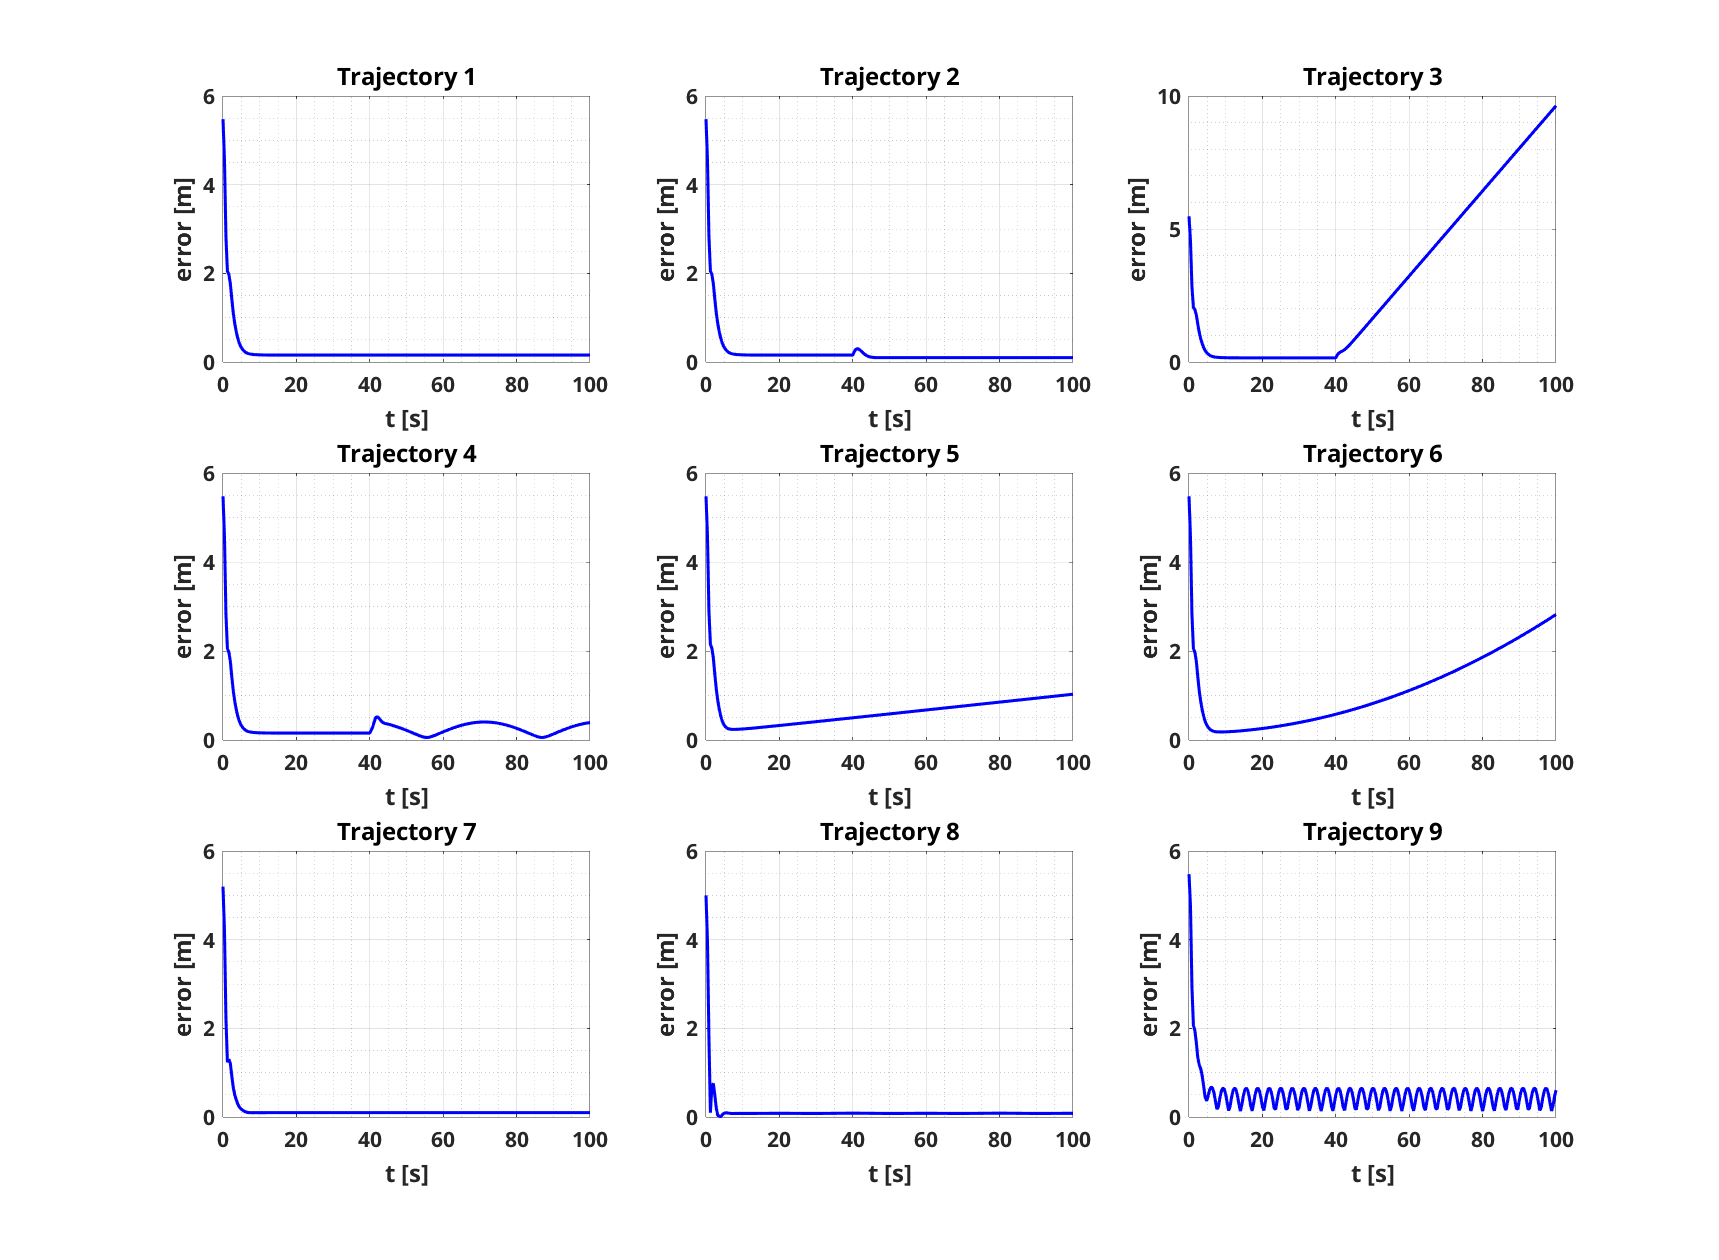
\includegraphics[width=0.98\textwidth]{error_all.png}
\caption{Position error against time for all trajectories.}\label{fig:errors}
\end{figure}

The straight and weaving paths (trajectories 7 and 8) are tracked to about a decimeter or better. The helix (trajectory 1) settles to a small, nearly constant offset. Trajectories 2 to 4 share the same first segment and differ after the transition to the straight run. The expanding spirals (5 and 6) and the accelerating climb (3) show errors that grow with the reference, while the oscillating cases (4 and 9) show bounded oscillating errors. The peak thrust and tilt are reached during the start-up correction and are largest for trajectory 9.

\subsection{Trajectory 1: Helix at constant radius and climb rate}\label{sec:t1}

The vehicle starts away from the reference, and the position error decays within the first few position periods to a small, nearly constant offset that persists for the rest of the run. Roll and pitch react strongly during the start-up correction and then settle to nearly constant small values, since the centripetal acceleration of the slow circle is small. The yaw angle increases at a constant rate, following the heading of the circular path, and the actual yaw is indistinguishable from the reference. After the transient the thrust equals the vehicle weight, the torques vanish and all four rotors run at the same constant speed. The extremes of the rotor speeds and of the thrust occur only during the first seconds.

\begin{figure}[H]
\centering
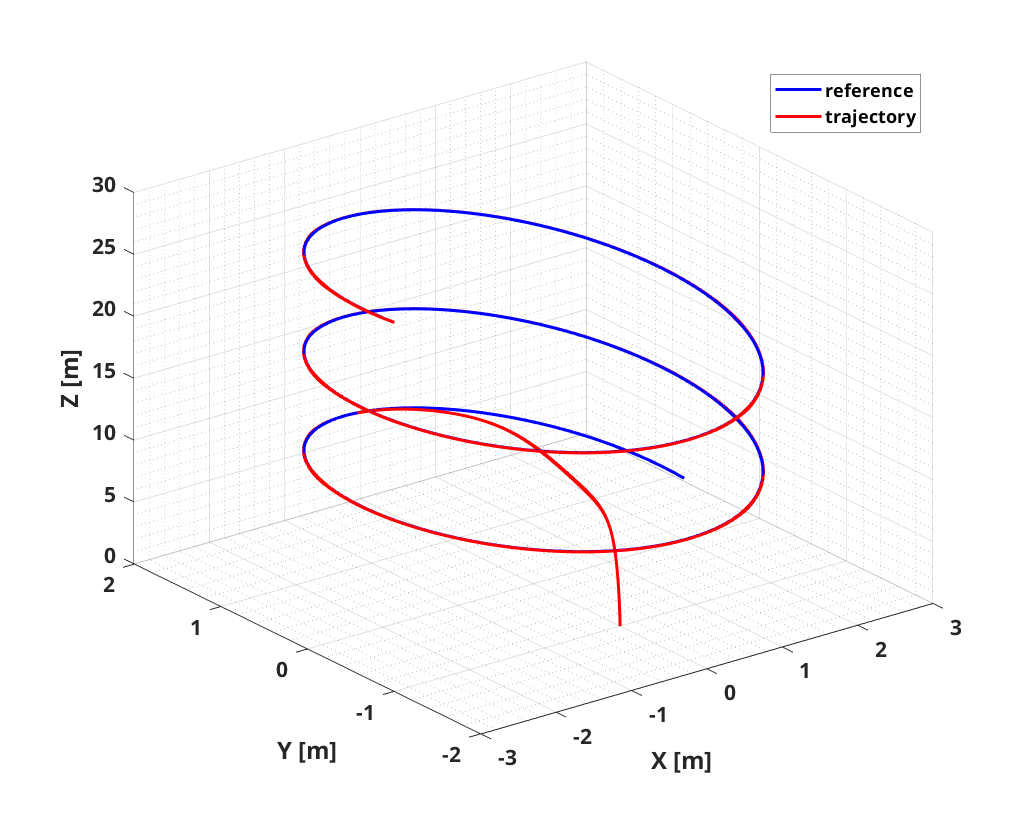
\includegraphics[width=0.72\textwidth]{traj1_path3d.png}
\caption{Trajectory 1: reference and flown path.}
\end{figure}

\begin{figure}[H]
\centering
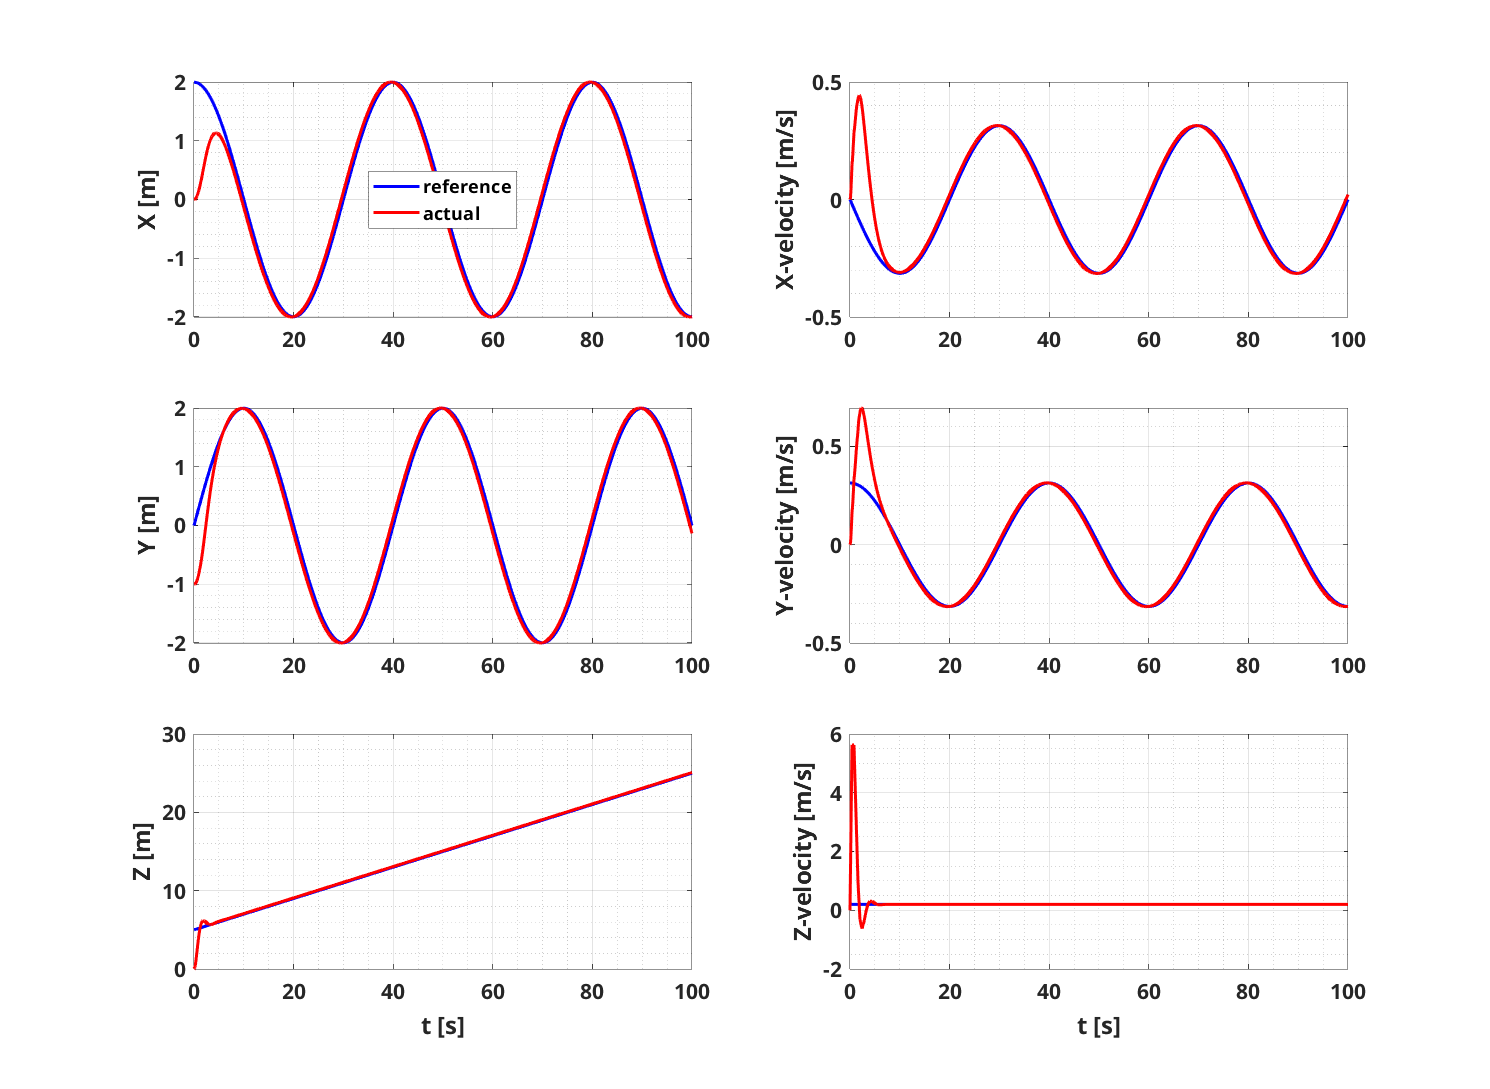
\includegraphics[width=0.95\textwidth]{traj1_position_velocity.png}
\caption{Trajectory 1: position and inertial velocity against reference.}
\end{figure}

\begin{figure}[H]
\centering
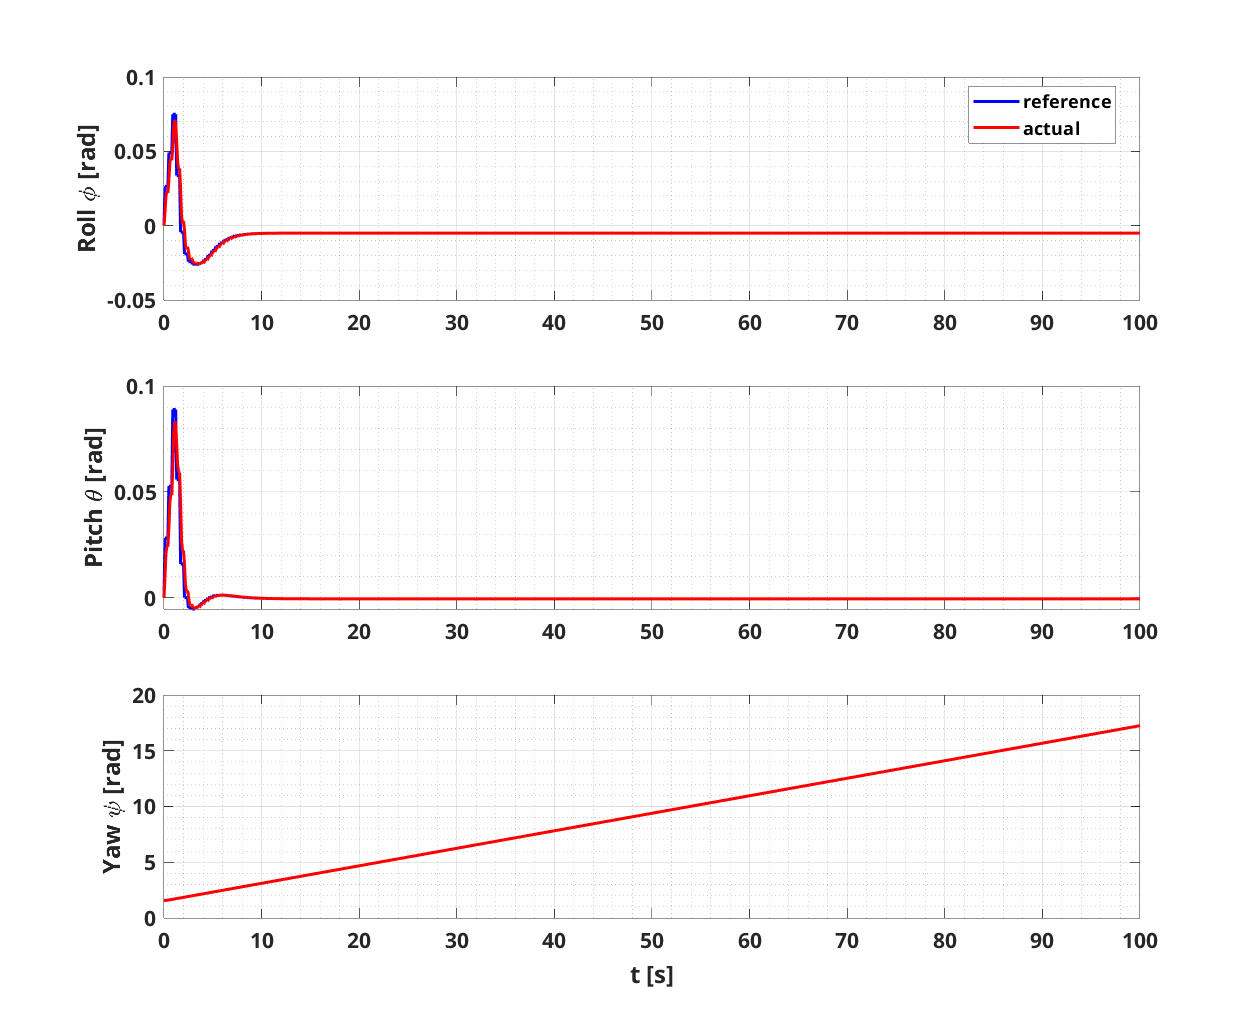
\includegraphics[width=0.95\textwidth]{traj1_attitude.png}
\caption{Trajectory 1: attitude angles against the references from the position loop.}
\end{figure}

\begin{figure}[H]
\centering
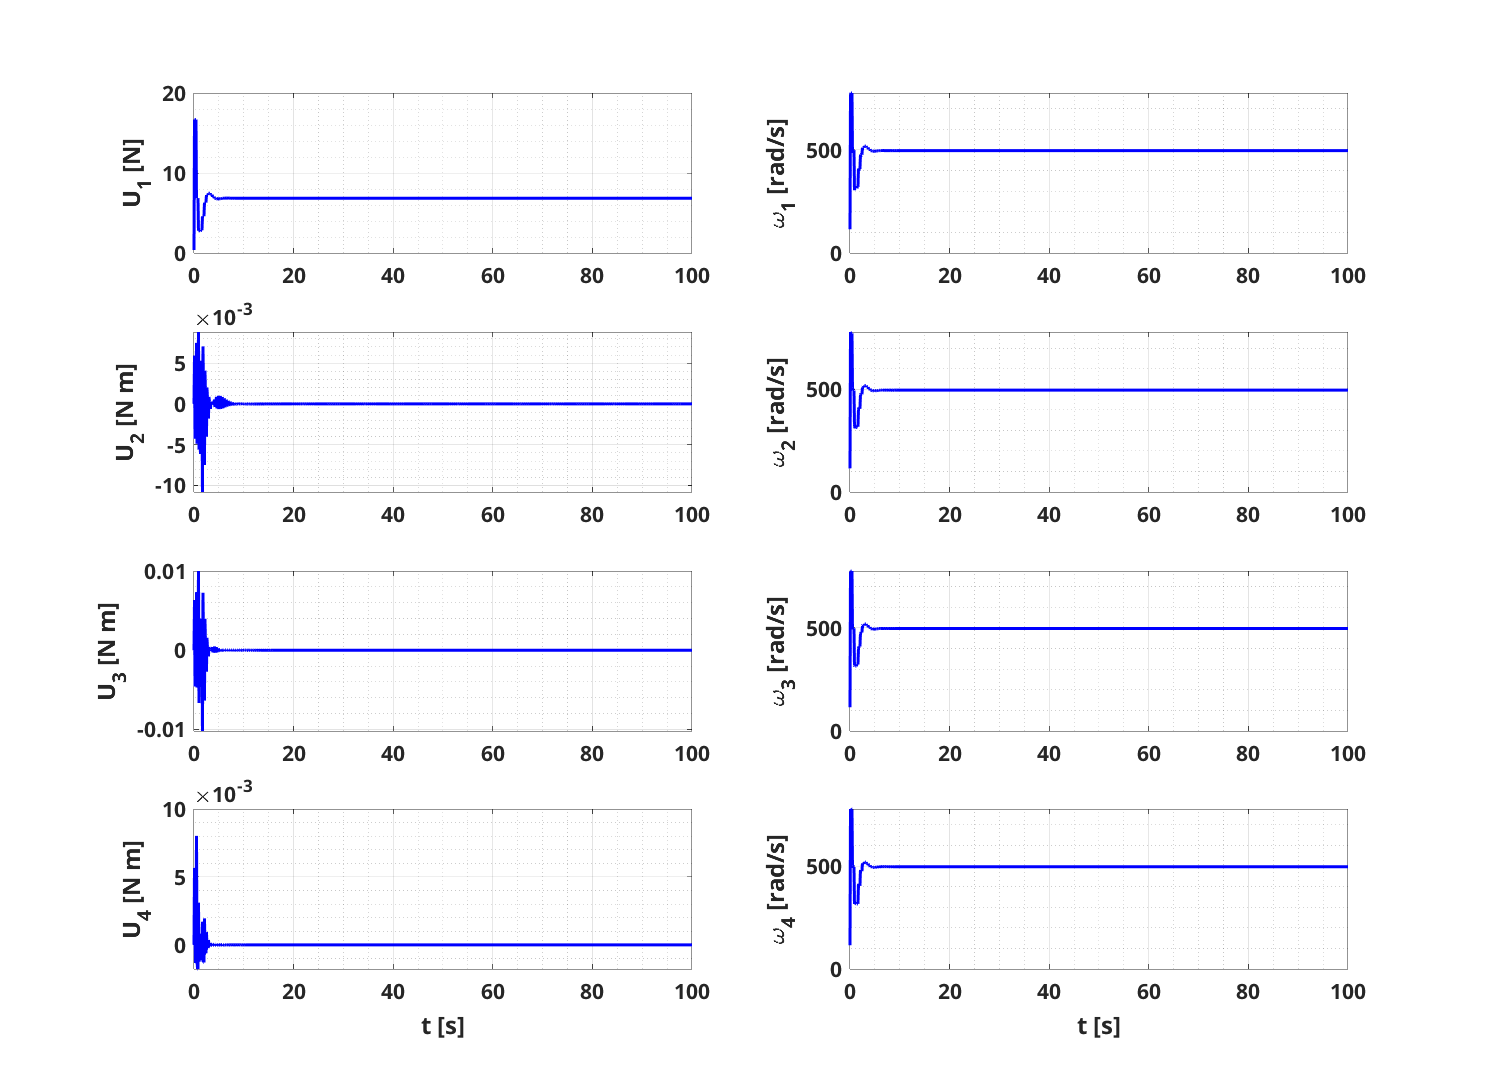
\includegraphics[width=0.95\textwidth]{traj1_inputs_rotors.png}
\caption{Trajectory 1: control inputs and rotor speeds.}
\end{figure}

\subsection{Trajectory 2: Circle followed by a straight run with constant climb}\label{sec:t2}

During the circular segment the behavior is the same as for the first trajectory. At the transition to the straight run the reference acceleration changes abruptly and the heading stops rotating. The position error shows a short bump, the roll, pitch and yaw references respond with a brief transient, and the yaw torque and the rotor speeds show a short spike. After the transition the vehicle settles again, and the error on the straight segment is smaller than on the circle.

\begin{figure}[H]
\centering
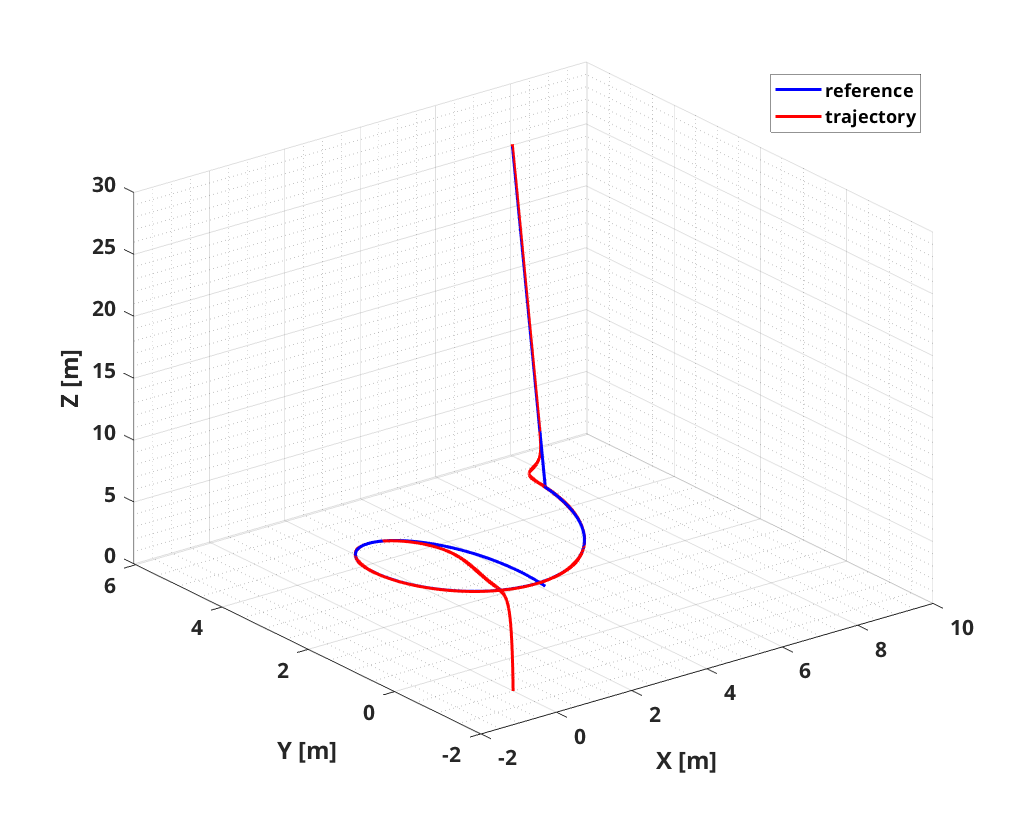
\includegraphics[width=0.72\textwidth]{traj2_path3d.png}
\caption{Trajectory 2: reference and flown path.}
\end{figure}

\begin{figure}[H]
\centering
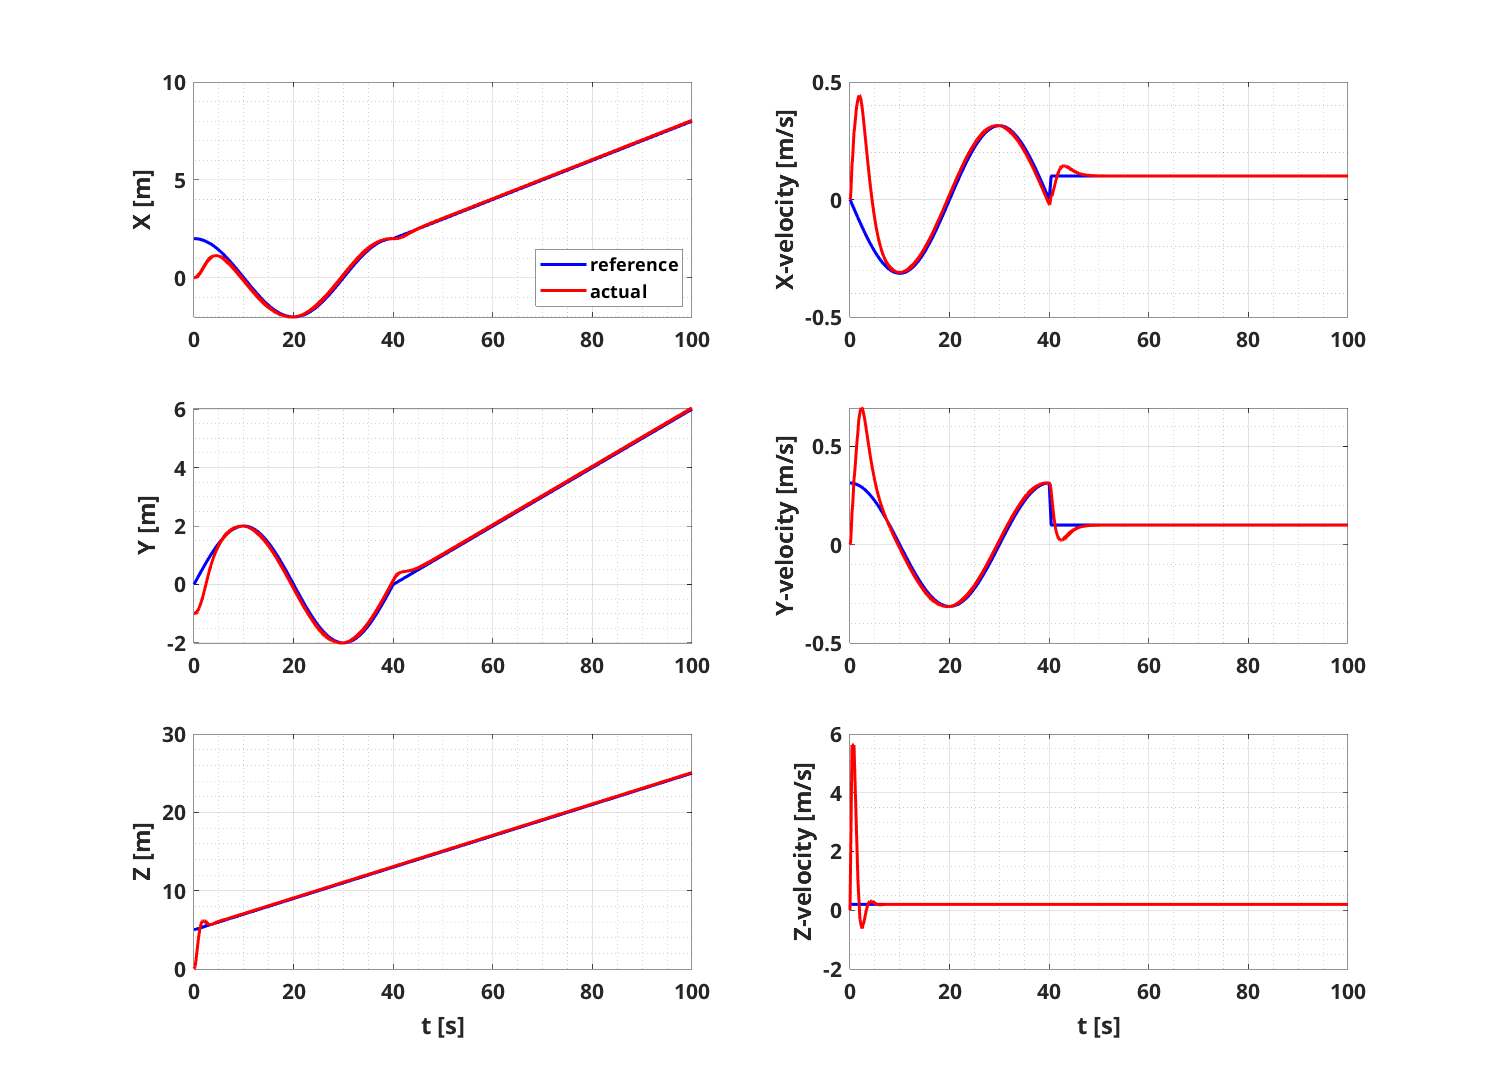
\includegraphics[width=0.95\textwidth]{traj2_position_velocity.png}
\caption{Trajectory 2: position and inertial velocity against reference.}
\end{figure}

\begin{figure}[H]
\centering
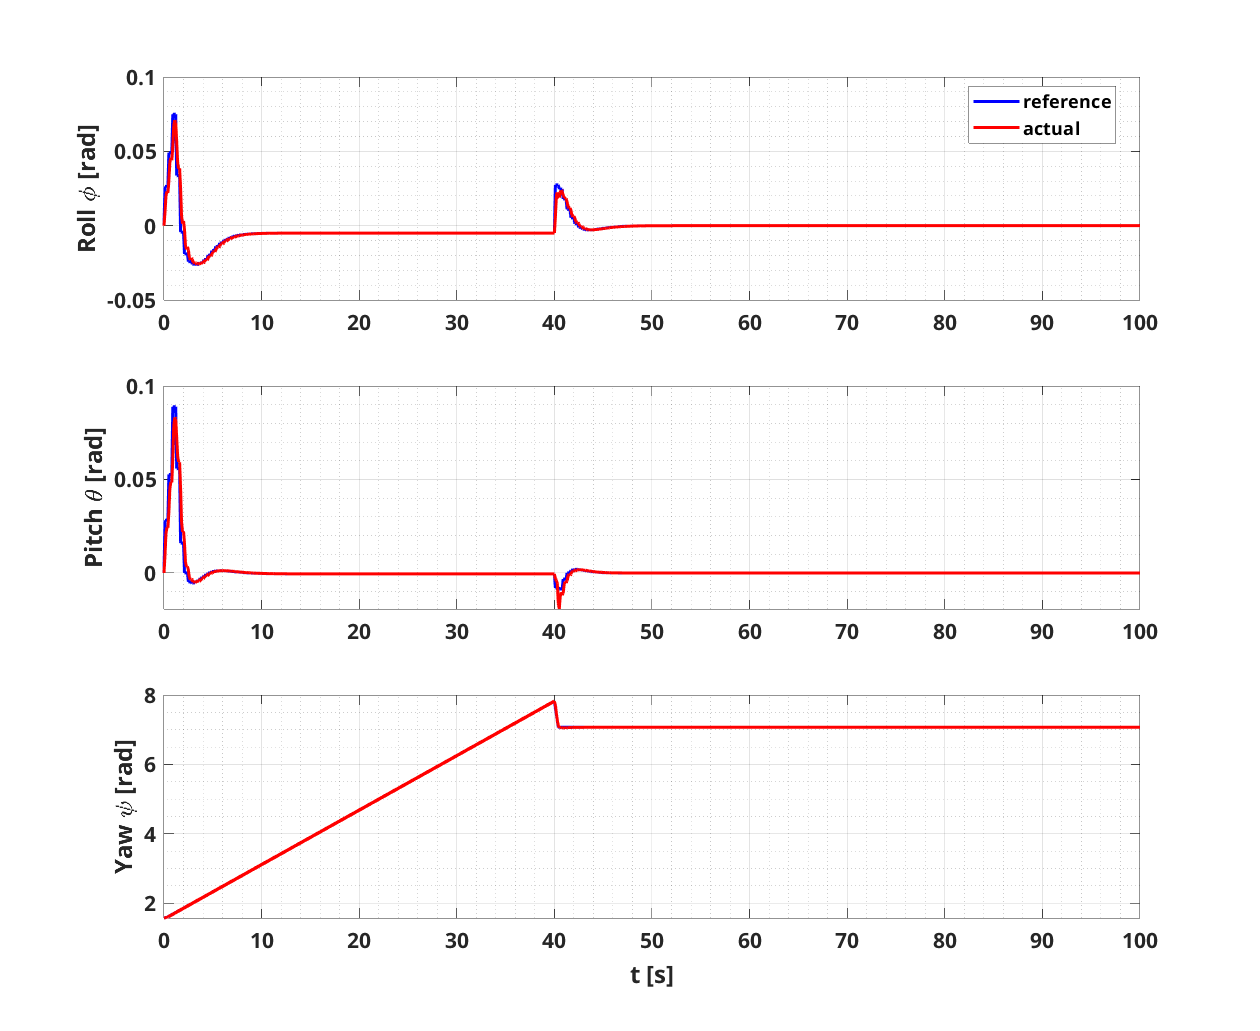
\includegraphics[width=0.95\textwidth]{traj2_attitude.png}
\caption{Trajectory 2: attitude angles against the references from the position loop.}
\end{figure}

\begin{figure}[H]
\centering
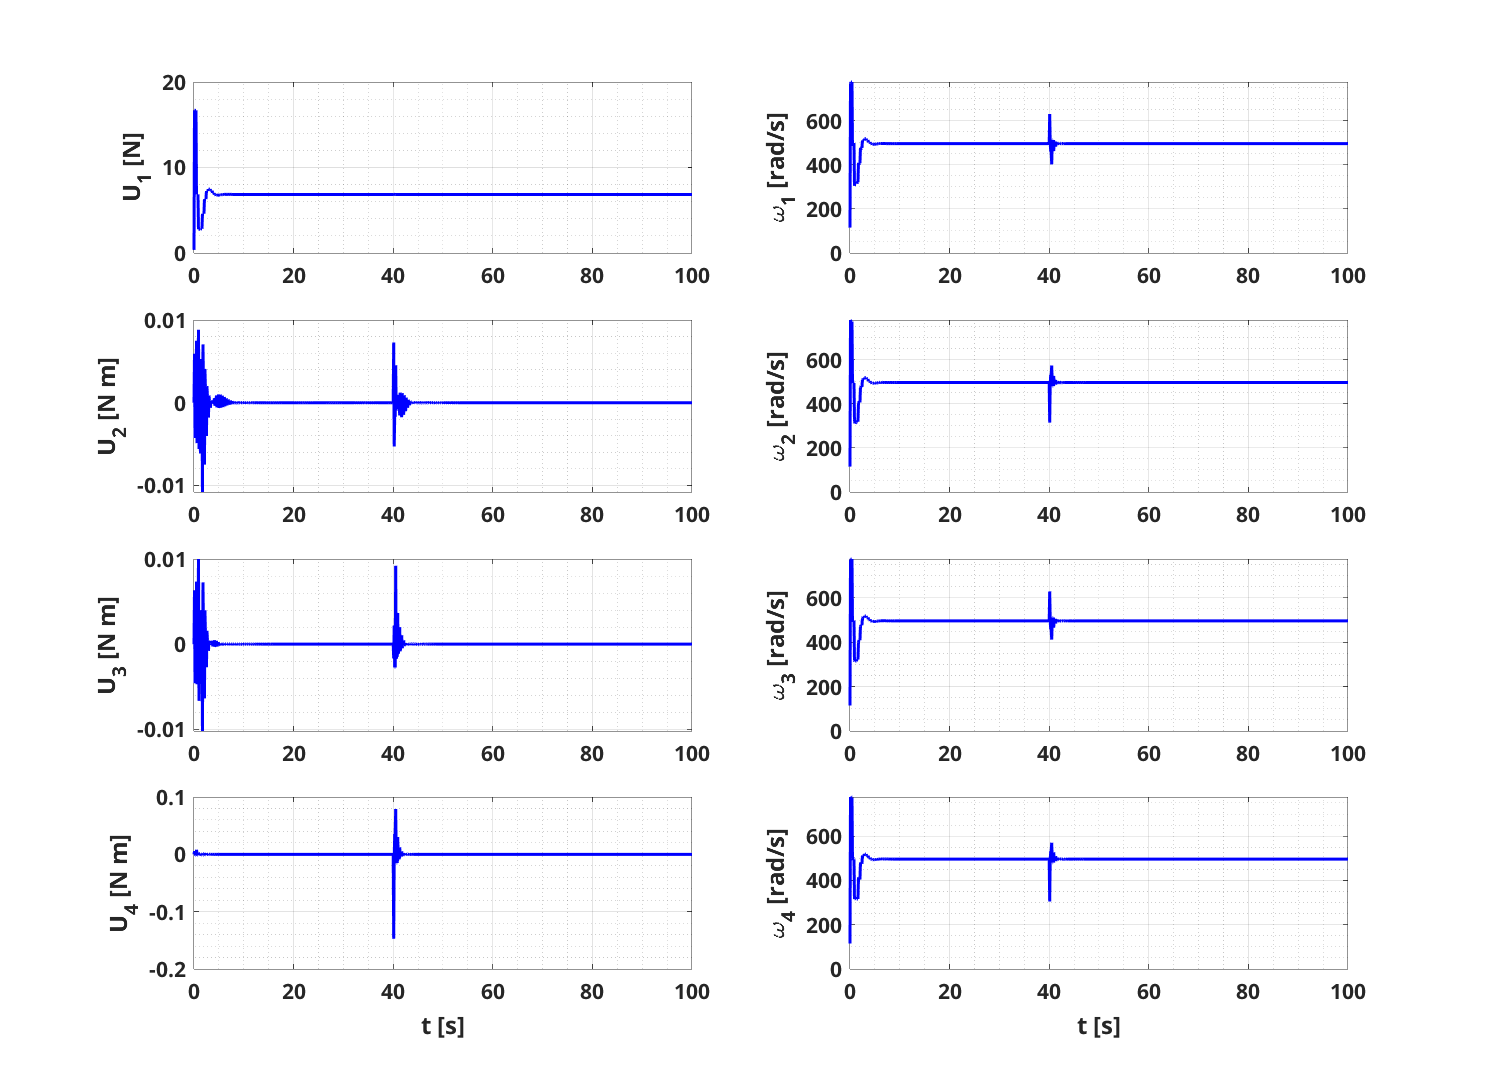
\includegraphics[width=0.95\textwidth]{traj2_inputs_rotors.png}
\caption{Trajectory 2: control inputs and rotor speeds.}
\end{figure}

\subsection{Trajectory 3: Circle followed by a straight run with quadratic climb}\label{sec:t3}

The first segment is identical to the previous case. After the transition the reference climbs with constant vertical acceleration to an altitude of several hundred meters, so its vertical speed keeps increasing. The vehicle follows, but the position error grows steadily with the climb speed and reaches its largest value at the end of the run. The thrust stays close to the vehicle weight throughout and the rotor speeds stay in a moderate range, so the growing error reflects the lag of a position loop without integral action behind an ever-accelerating reference, not a loss of stability or actuator saturation.

\begin{figure}[H]
\centering
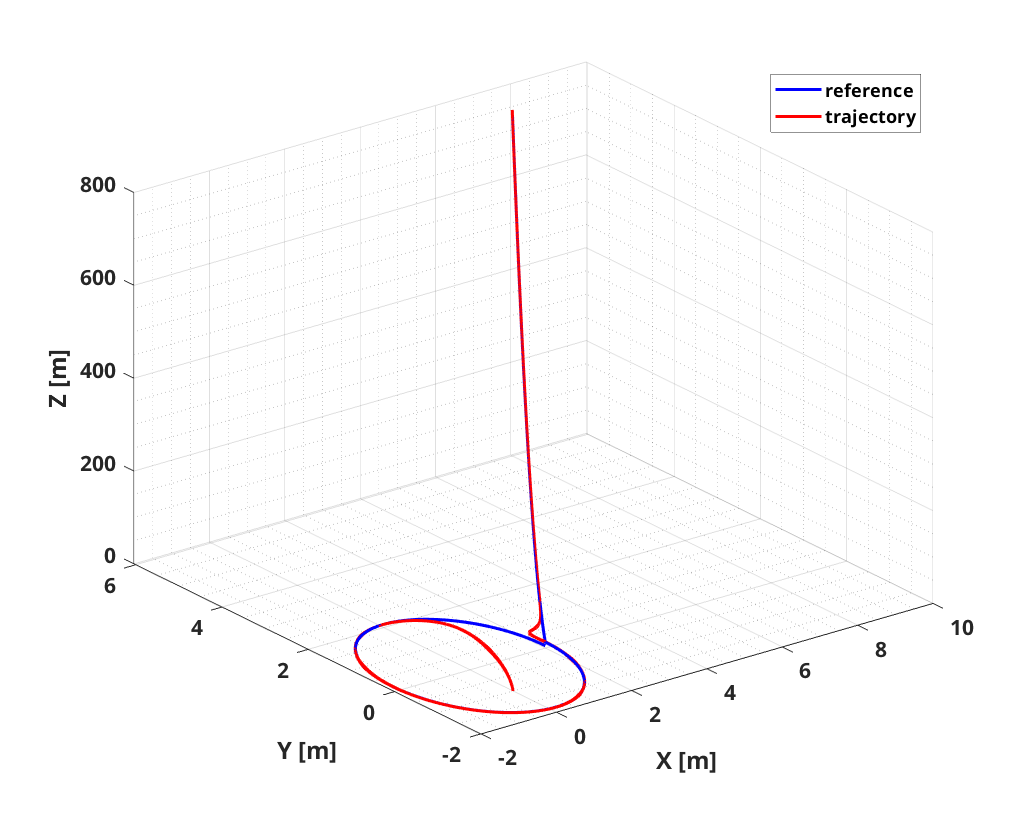
\includegraphics[width=0.72\textwidth]{traj3_path3d.png}
\caption{Trajectory 3: reference and flown path.}
\end{figure}

\begin{figure}[H]
\centering
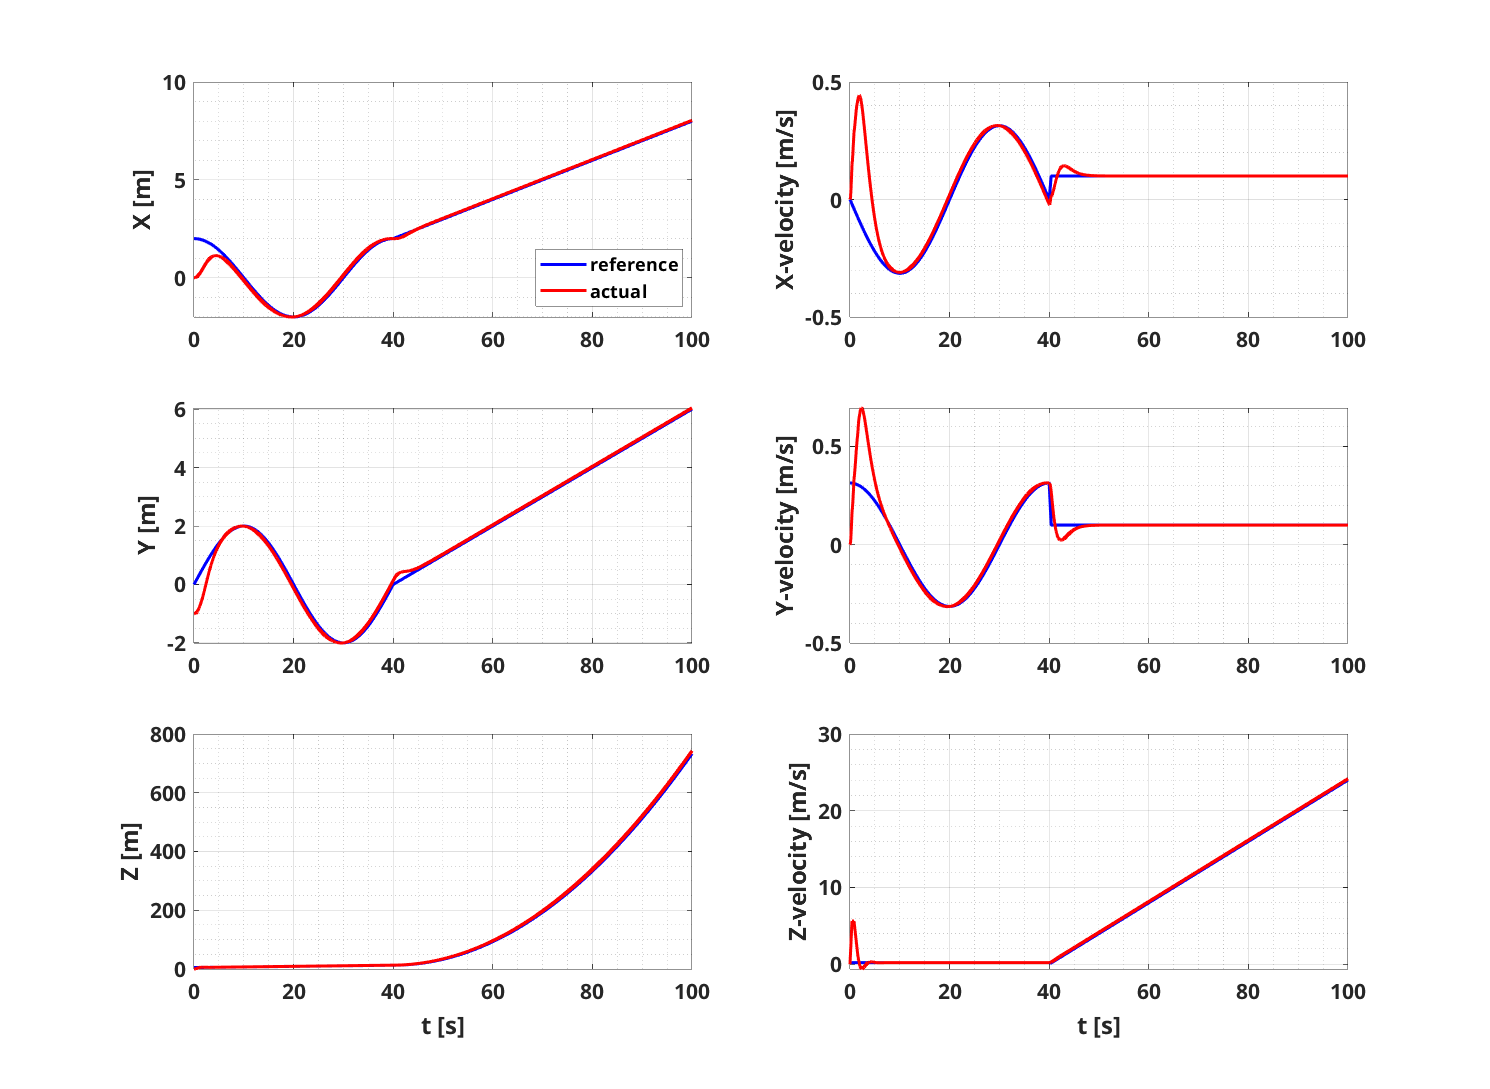
\includegraphics[width=0.95\textwidth]{traj3_position_velocity.png}
\caption{Trajectory 3: position and inertial velocity against reference.}
\end{figure}

\begin{figure}[H]
\centering
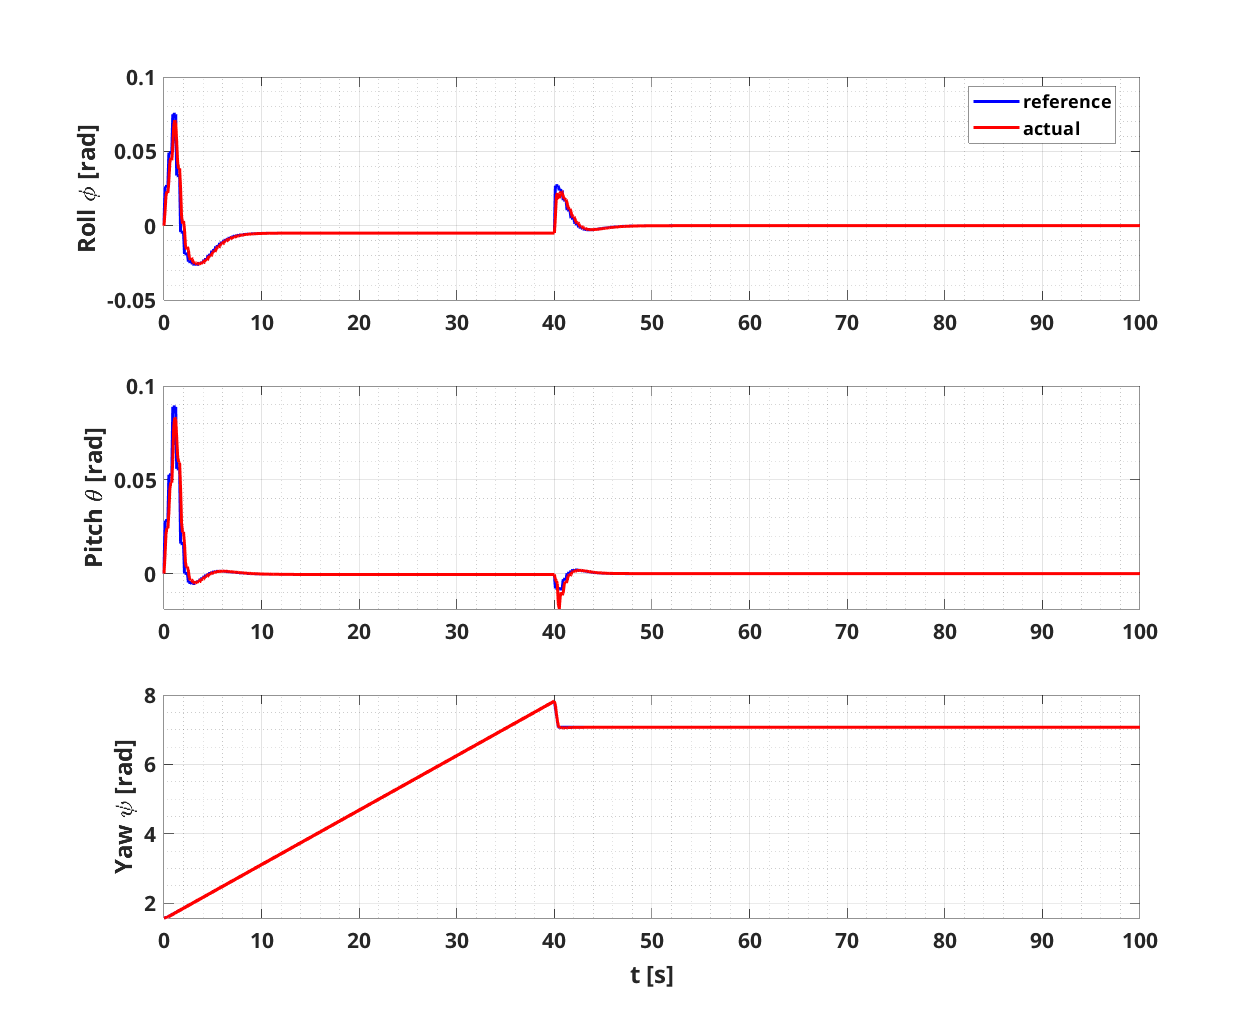
\includegraphics[width=0.95\textwidth]{traj3_attitude.png}
\caption{Trajectory 3: attitude angles against the references from the position loop.}
\end{figure}

\begin{figure}[H]
\centering
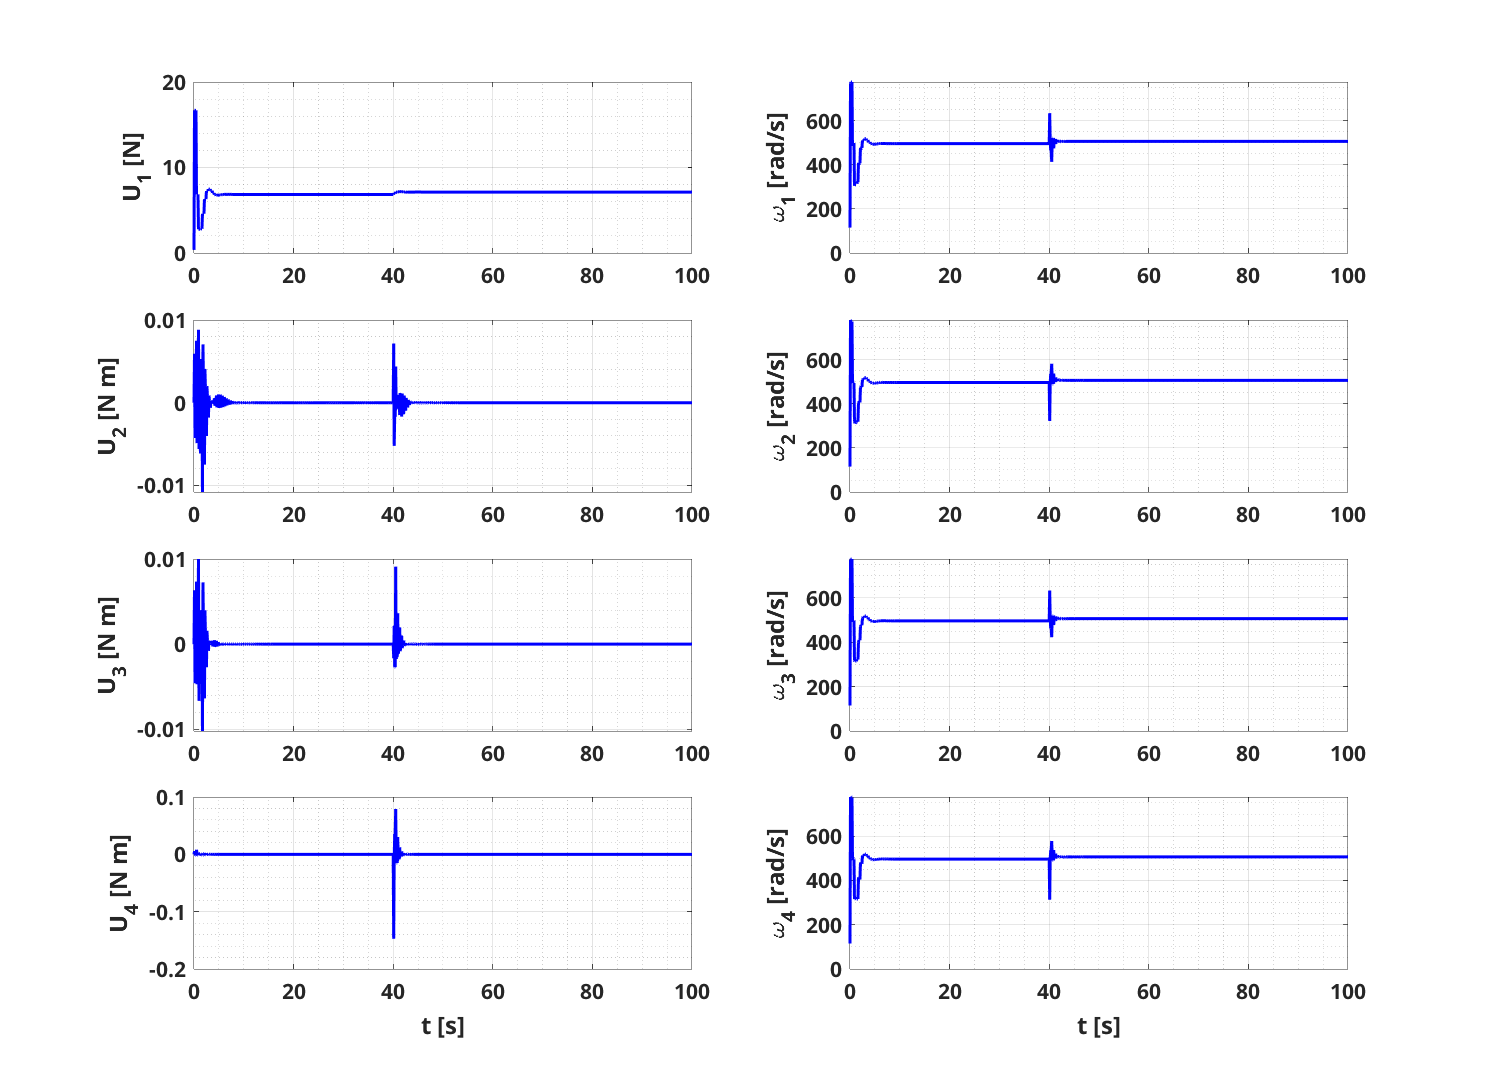
\includegraphics[width=0.95\textwidth]{traj3_inputs_rotors.png}
\caption{Trajectory 3: control inputs and rotor speeds.}
\end{figure}

\subsection{Trajectory 4: Circle followed by a straight run with sinusoidal climb}\label{sec:t4}

After the transition the reference climbs and descends sinusoidally. The error settles into a slow oscillation at the frequency of the vertical motion, with an amplitude of a few decimeters. The thrust oscillates about the weight, and the transition produces the same short transient in the attitude references and in the yaw torque as in the other two cases.

\begin{figure}[H]
\centering
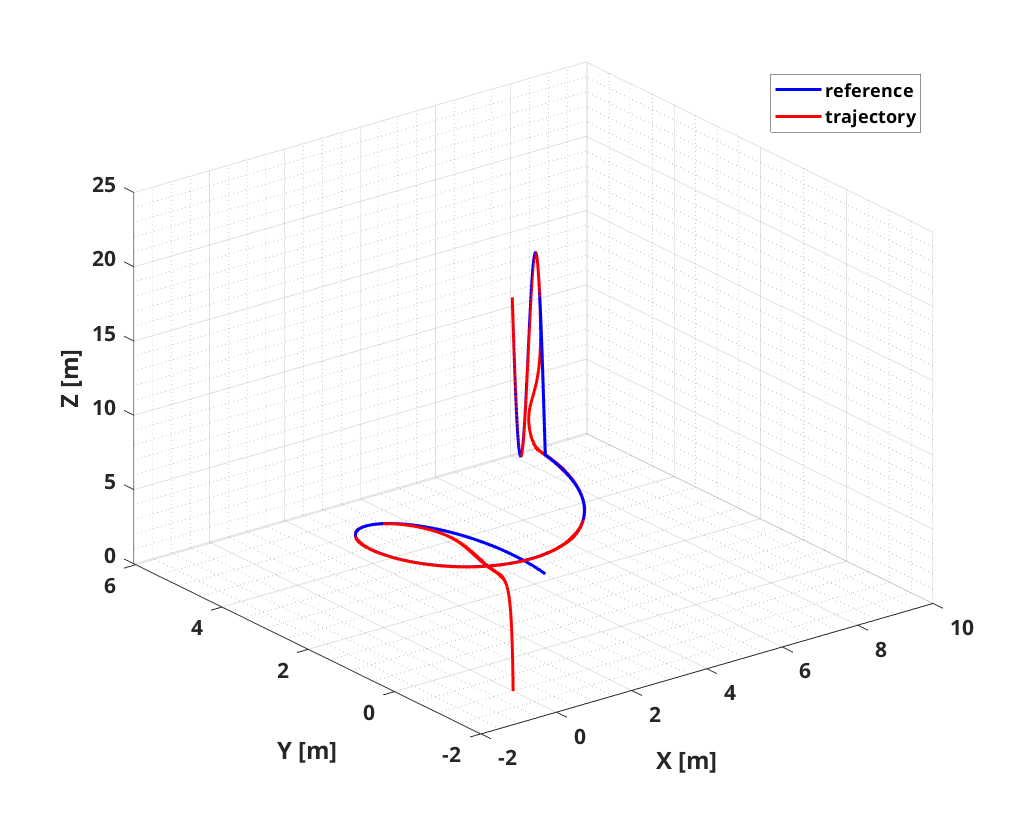
\includegraphics[width=0.72\textwidth]{traj4_path3d.png}
\caption{Trajectory 4: reference and flown path.}
\end{figure}

\begin{figure}[H]
\centering
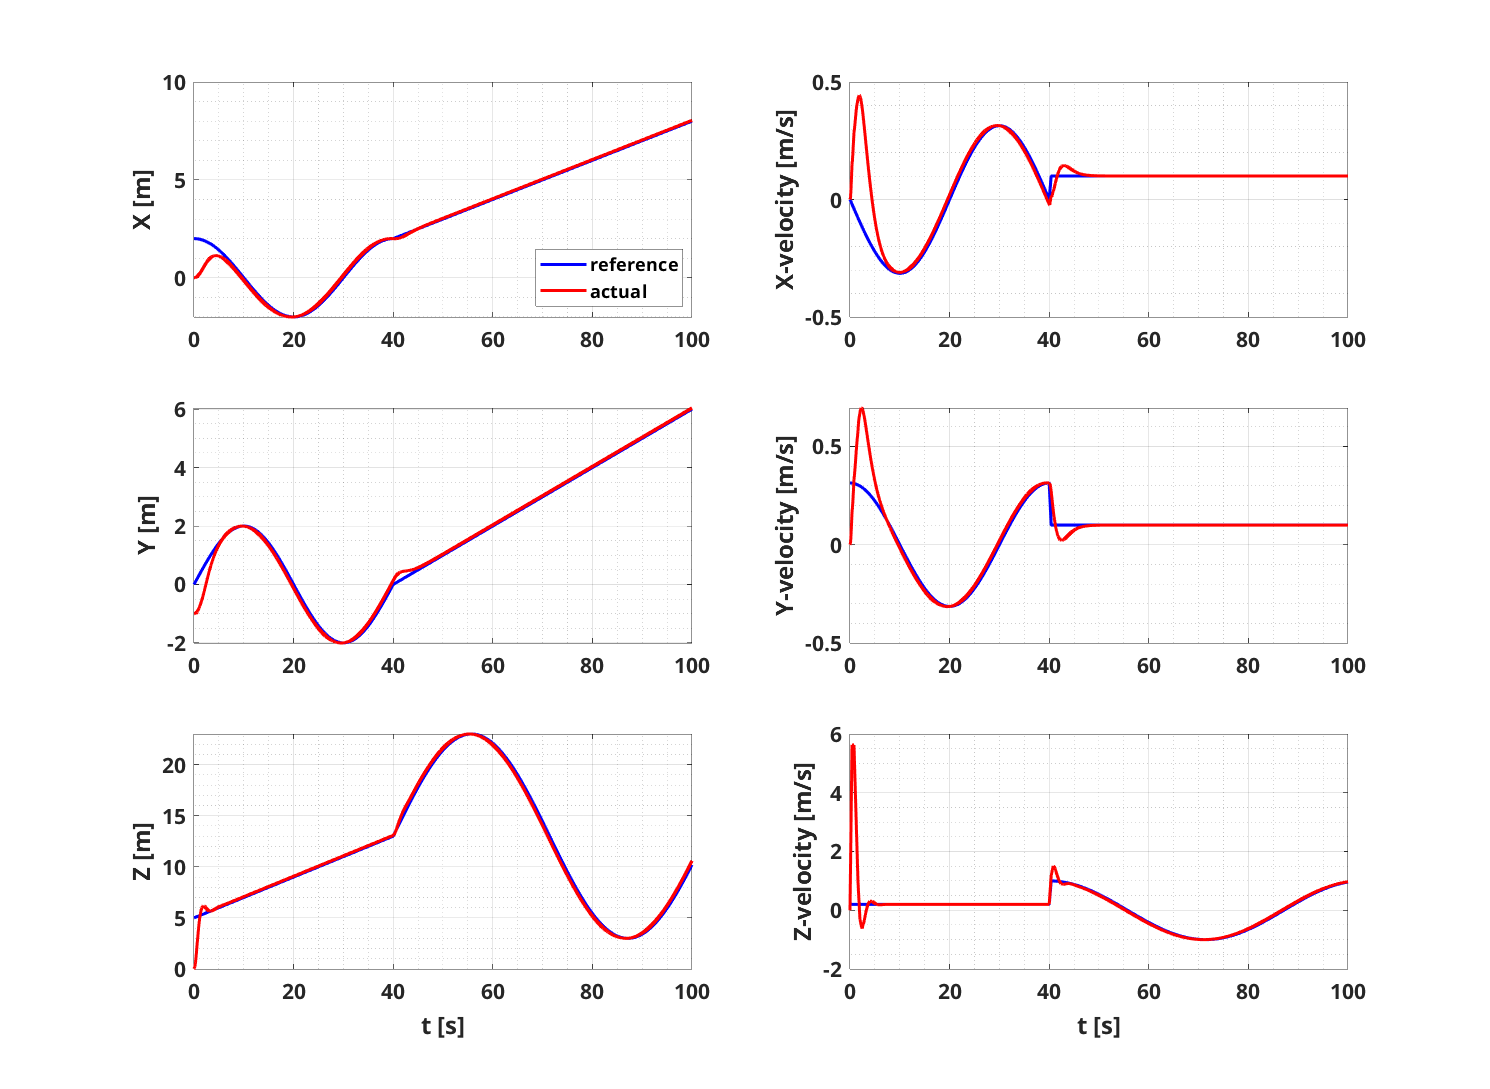
\includegraphics[width=0.95\textwidth]{traj4_position_velocity.png}
\caption{Trajectory 4: position and inertial velocity against reference.}
\end{figure}

\begin{figure}[H]
\centering
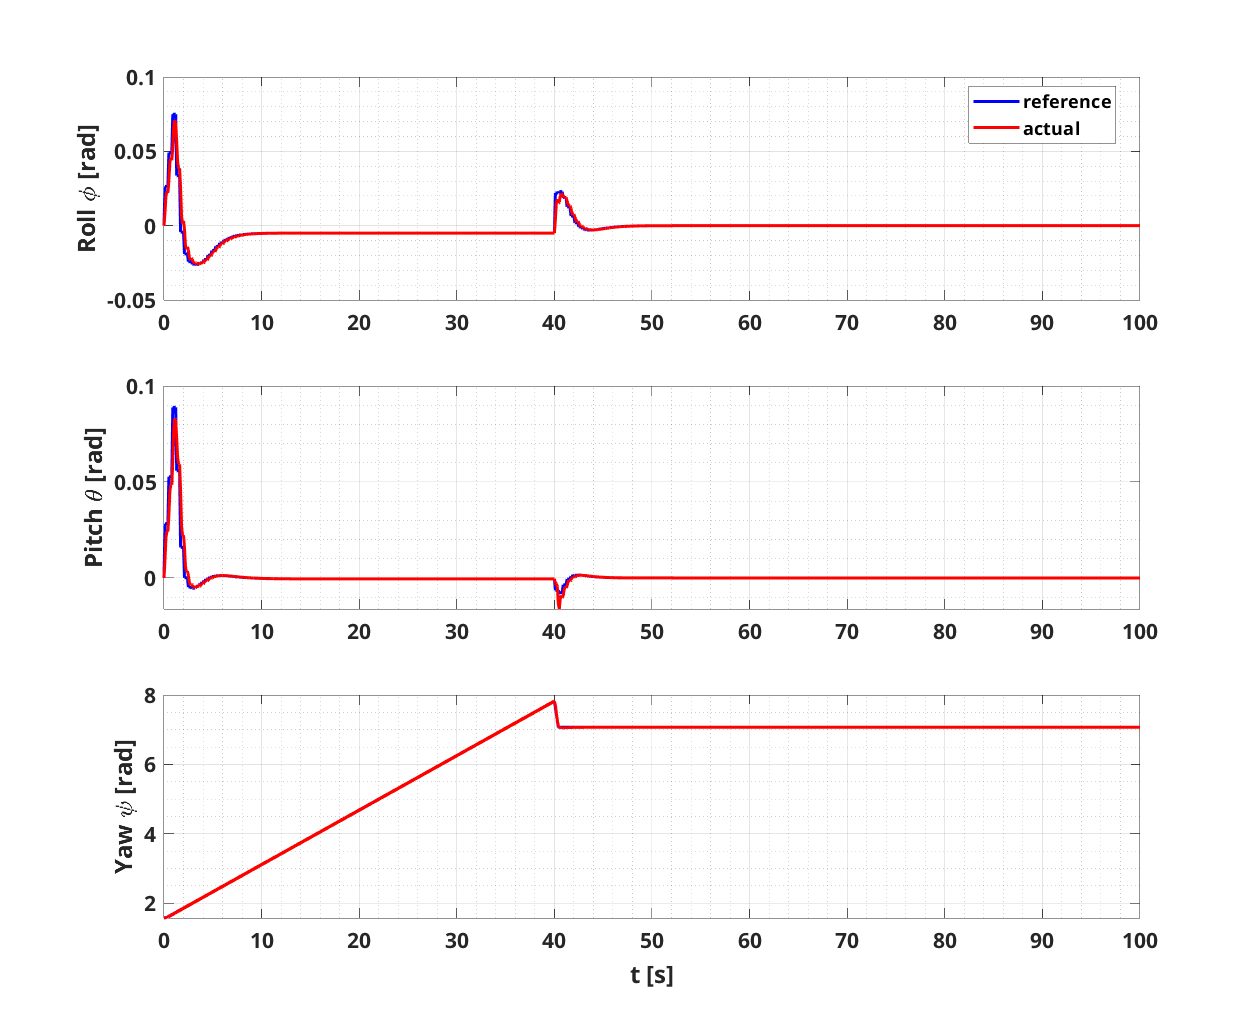
\includegraphics[width=0.95\textwidth]{traj4_attitude.png}
\caption{Trajectory 4: attitude angles against the references from the position loop.}
\end{figure}

\begin{figure}[H]
\centering
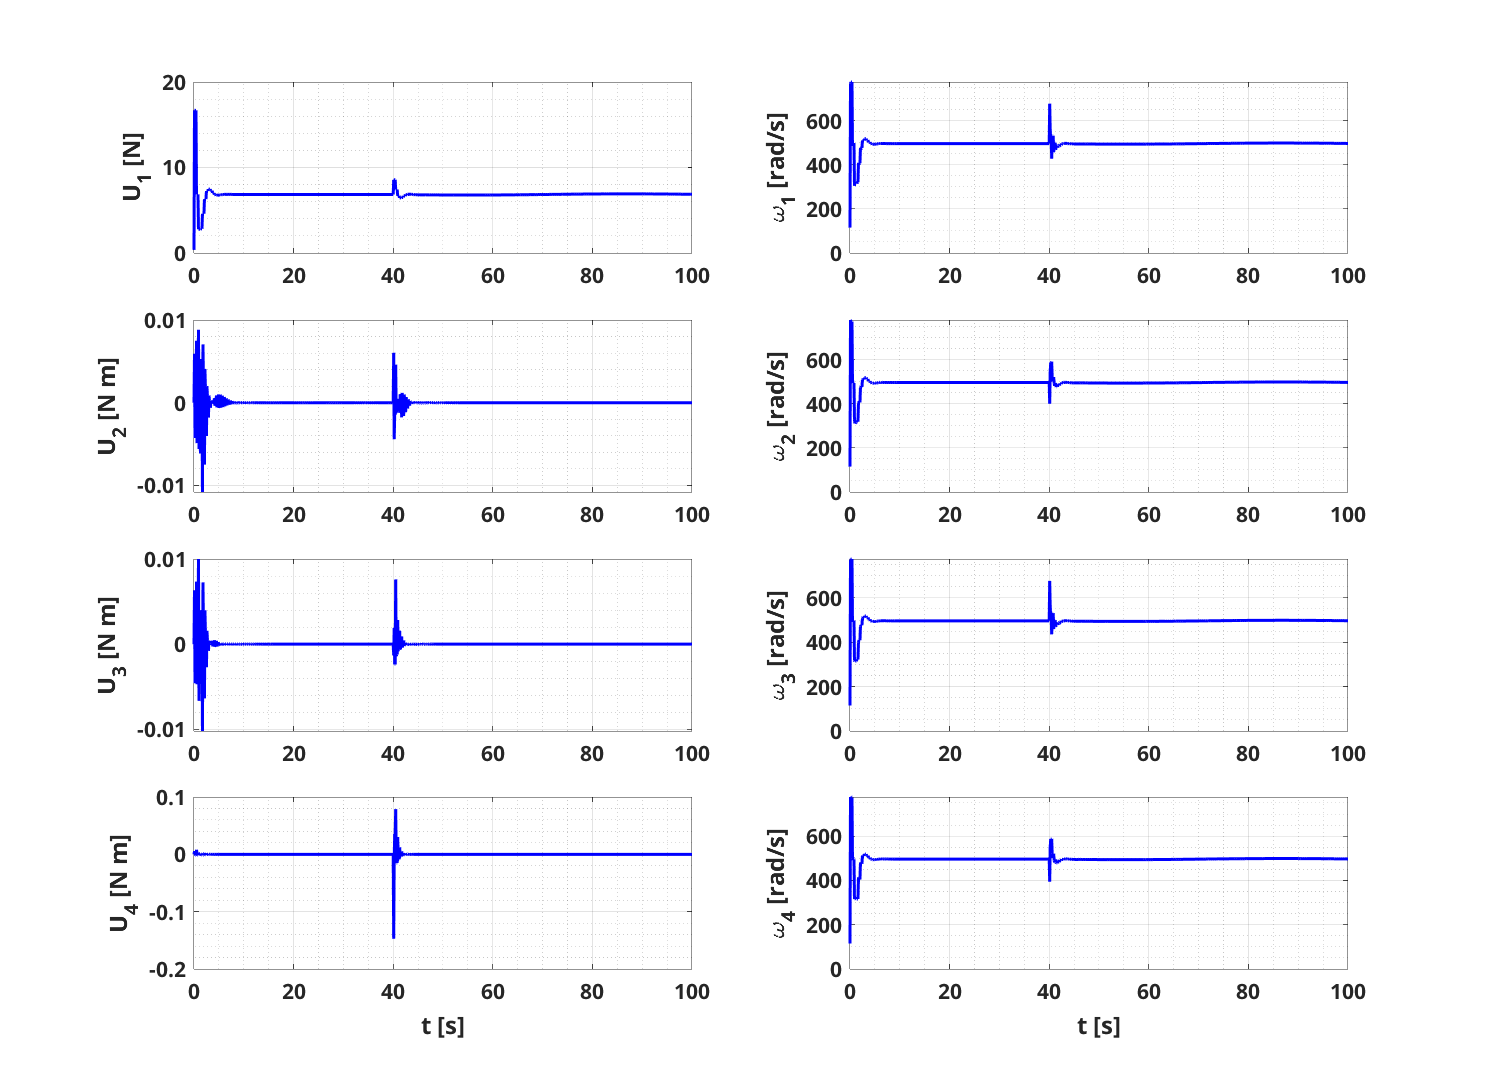
\includegraphics[width=0.95\textwidth]{traj4_inputs_rotors.png}
\caption{Trajectory 4: control inputs and rotor speeds.}
\end{figure}

\subsection{Trajectory 5: Helix with linearly growing radius}\label{sec:t5}

As the radius grows, the horizontal speed and the centripetal acceleration of the reference grow with it. The position error increases roughly linearly with time and reaches about one meter at the end of the run. The roll reference drifts slowly to larger negative values as the required centripetal acceleration increases, while the pitch stays small. The inputs remain smooth.

\begin{figure}[H]
\centering
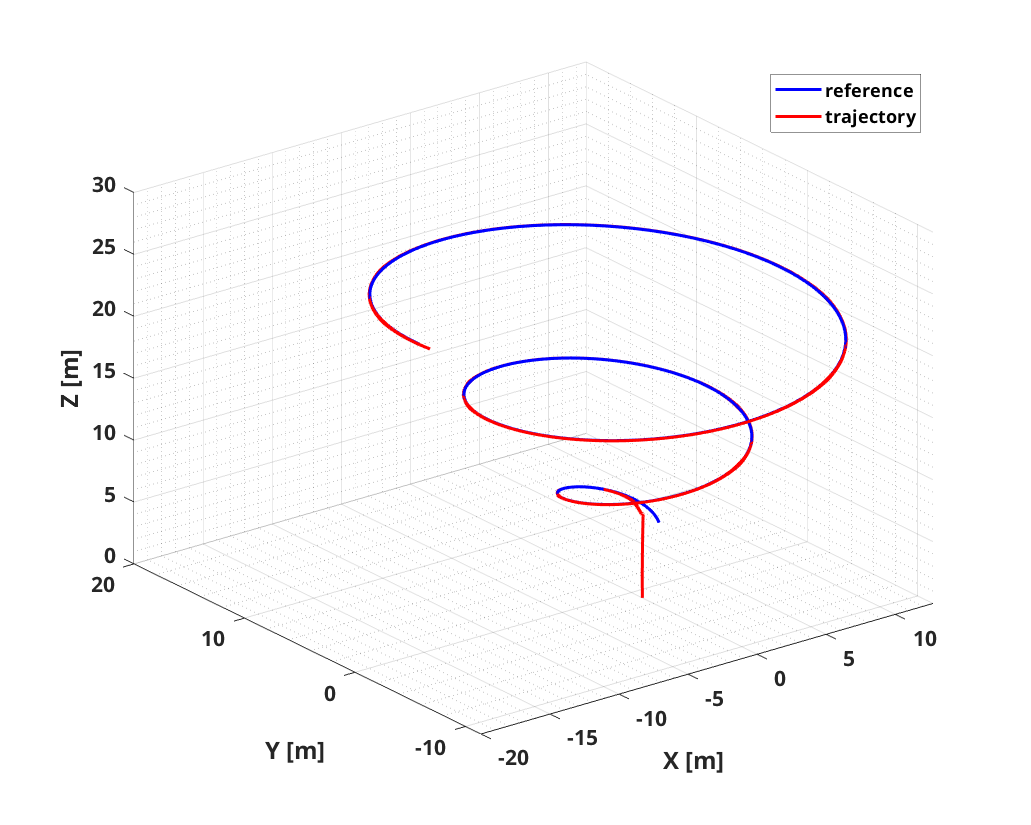
\includegraphics[width=0.72\textwidth]{traj5_path3d.png}
\caption{Trajectory 5: reference and flown path.}
\end{figure}

\begin{figure}[H]
\centering
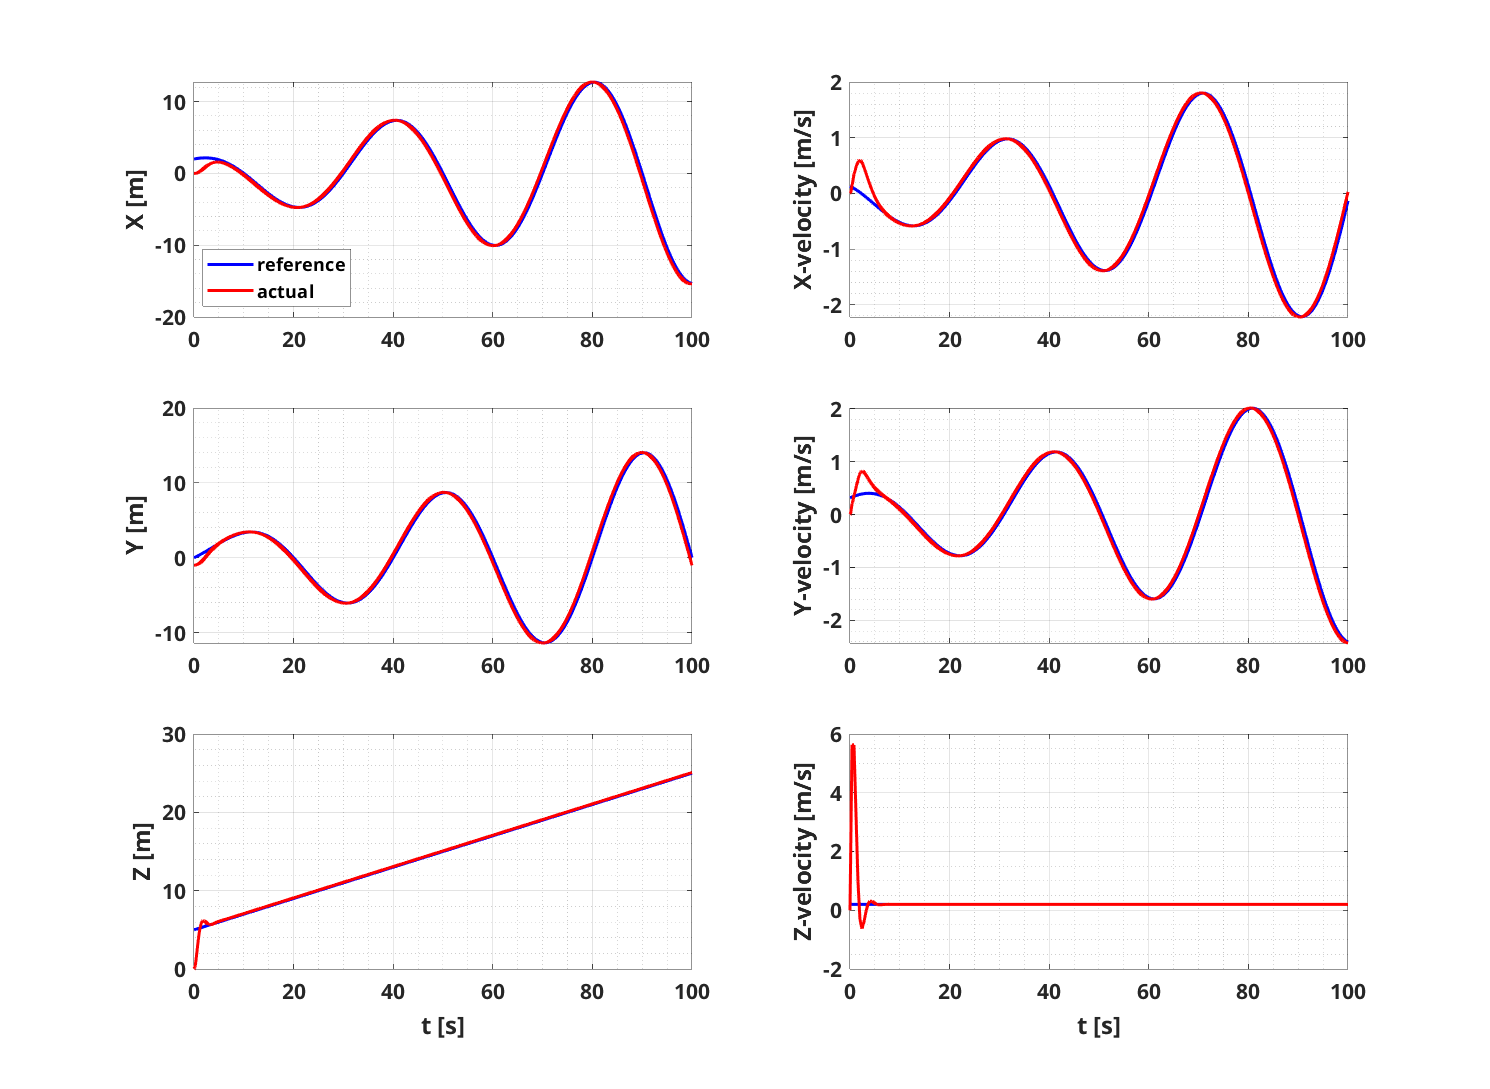
\includegraphics[width=0.95\textwidth]{traj5_position_velocity.png}
\caption{Trajectory 5: position and inertial velocity against reference.}
\end{figure}

\begin{figure}[H]
\centering
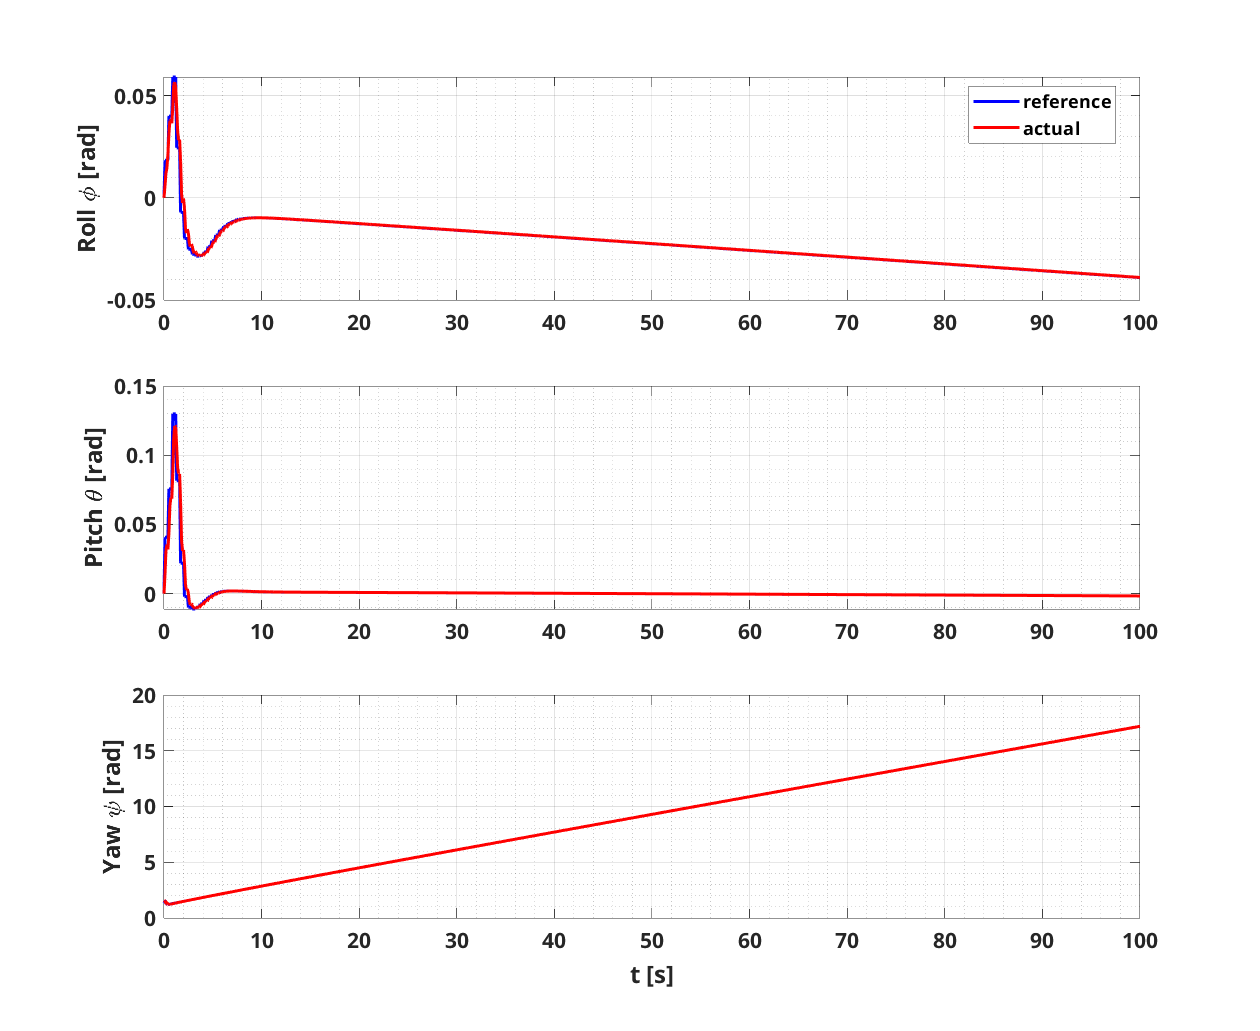
\includegraphics[width=0.95\textwidth]{traj5_attitude.png}
\caption{Trajectory 5: attitude angles against the references from the position loop.}
\end{figure}

\begin{figure}[H]
\centering
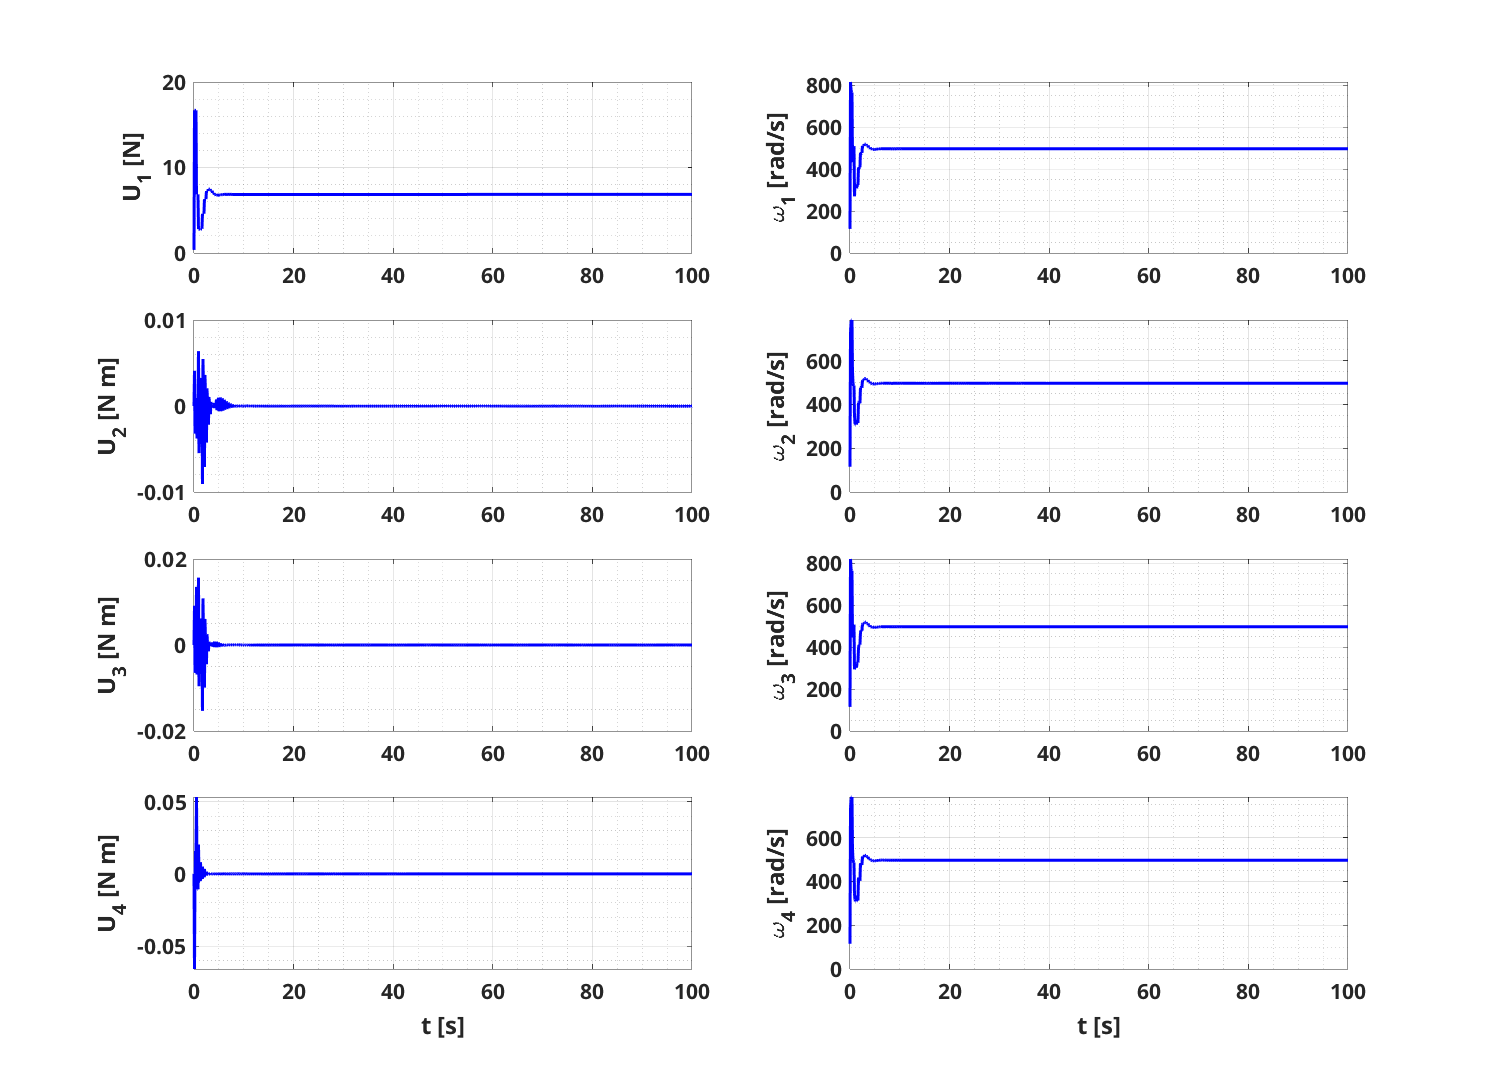
\includegraphics[width=0.95\textwidth]{traj5_inputs_rotors.png}
\caption{Trajectory 5: control inputs and rotor speeds.}
\end{figure}

\subsection{Trajectory 6: Helix with quadratically growing radius}\label{sec:t6}

The radius, and with it the horizontal speed and acceleration, grows faster than in the previous case, and the position error grows faster than linearly with time, reaching a few meters at the end. The roll angle drifts to the largest steady values of the helical cases, of the order of a tenth of a radian by the end of the run, which is still well inside the small-angle regime of the prediction model.

\begin{figure}[H]
\centering
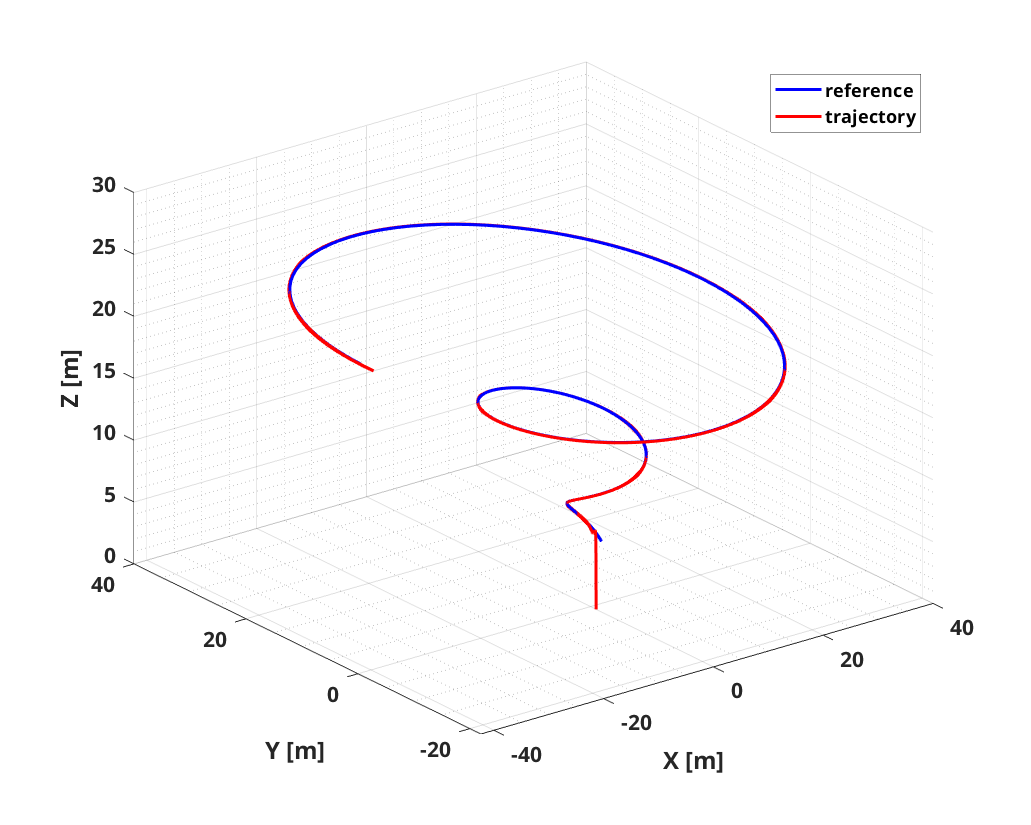
\includegraphics[width=0.72\textwidth]{traj6_path3d.png}
\caption{Trajectory 6: reference and flown path.}
\end{figure}

\begin{figure}[H]
\centering
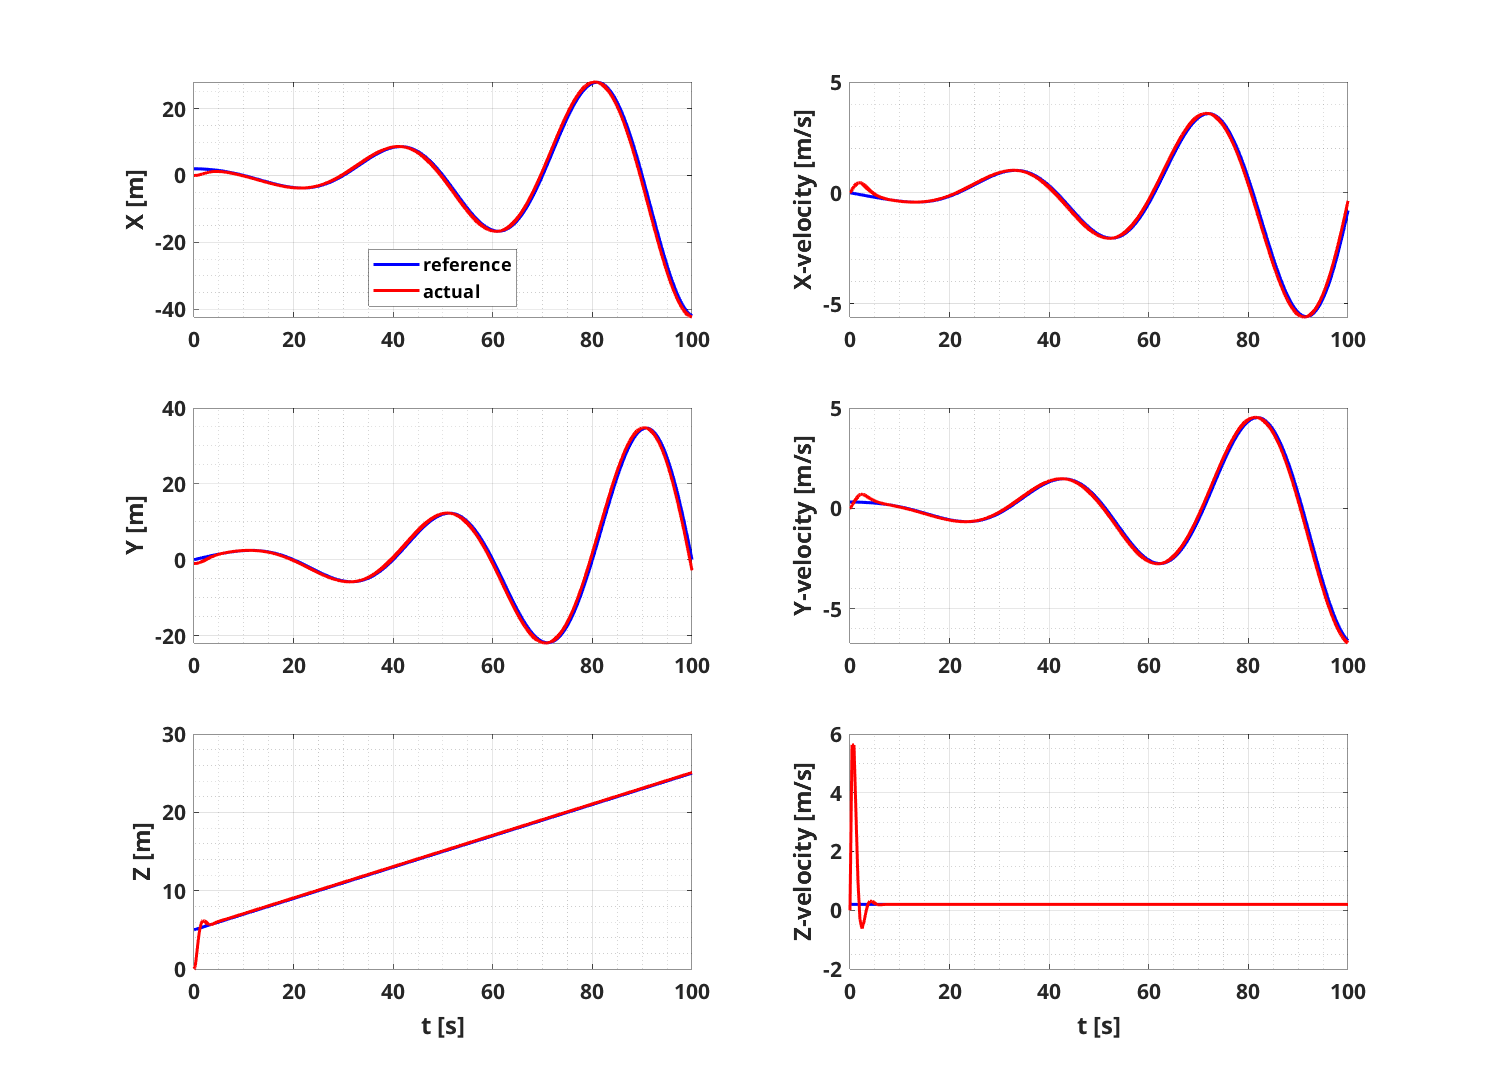
\includegraphics[width=0.95\textwidth]{traj6_position_velocity.png}
\caption{Trajectory 6: position and inertial velocity against reference.}
\end{figure}

\begin{figure}[H]
\centering
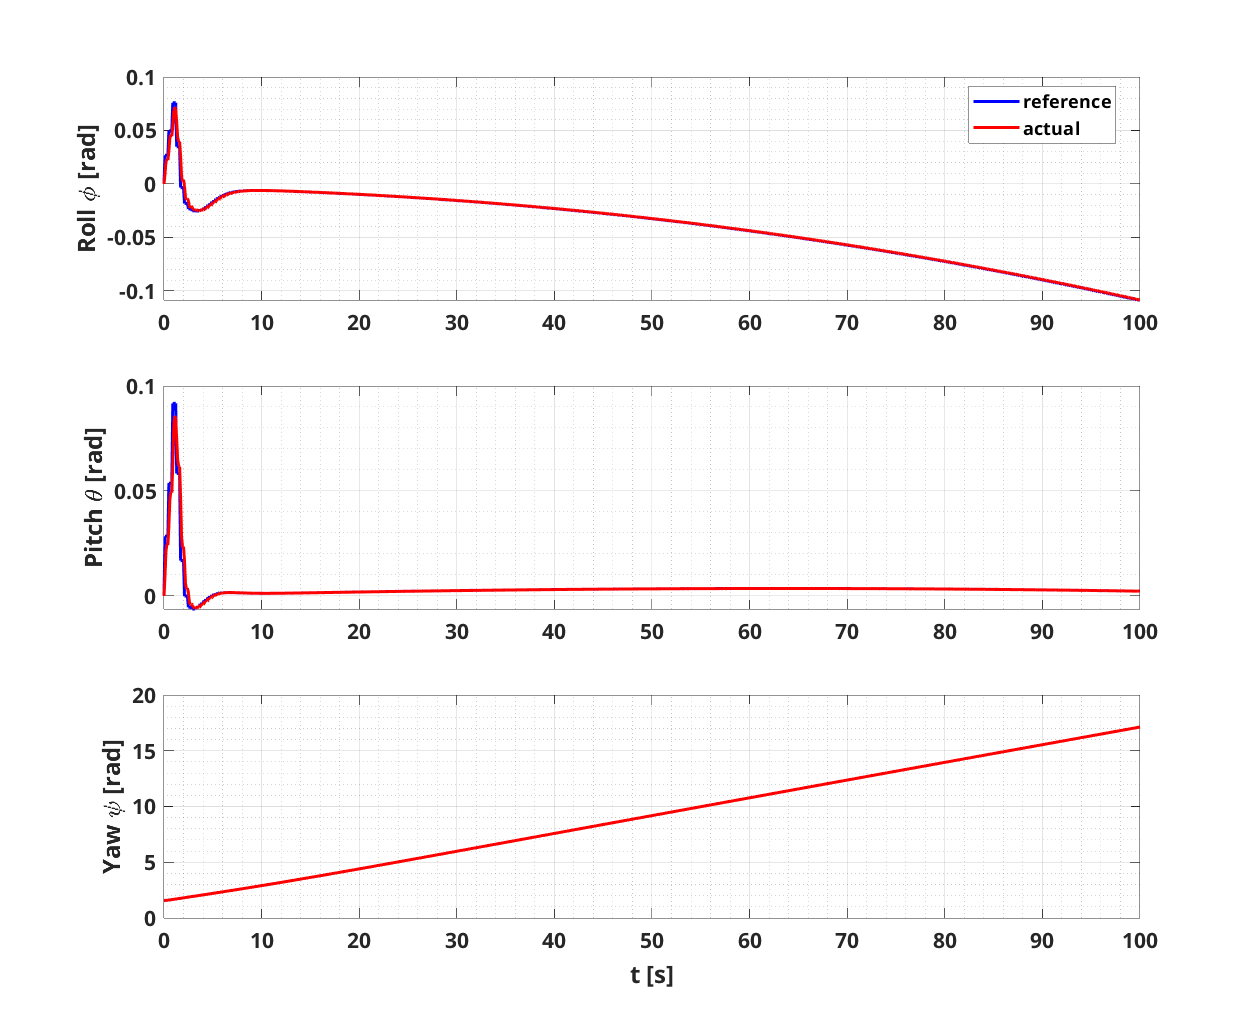
\includegraphics[width=0.95\textwidth]{traj6_attitude.png}
\caption{Trajectory 6: attitude angles against the references from the position loop.}
\end{figure}

\begin{figure}[H]
\centering
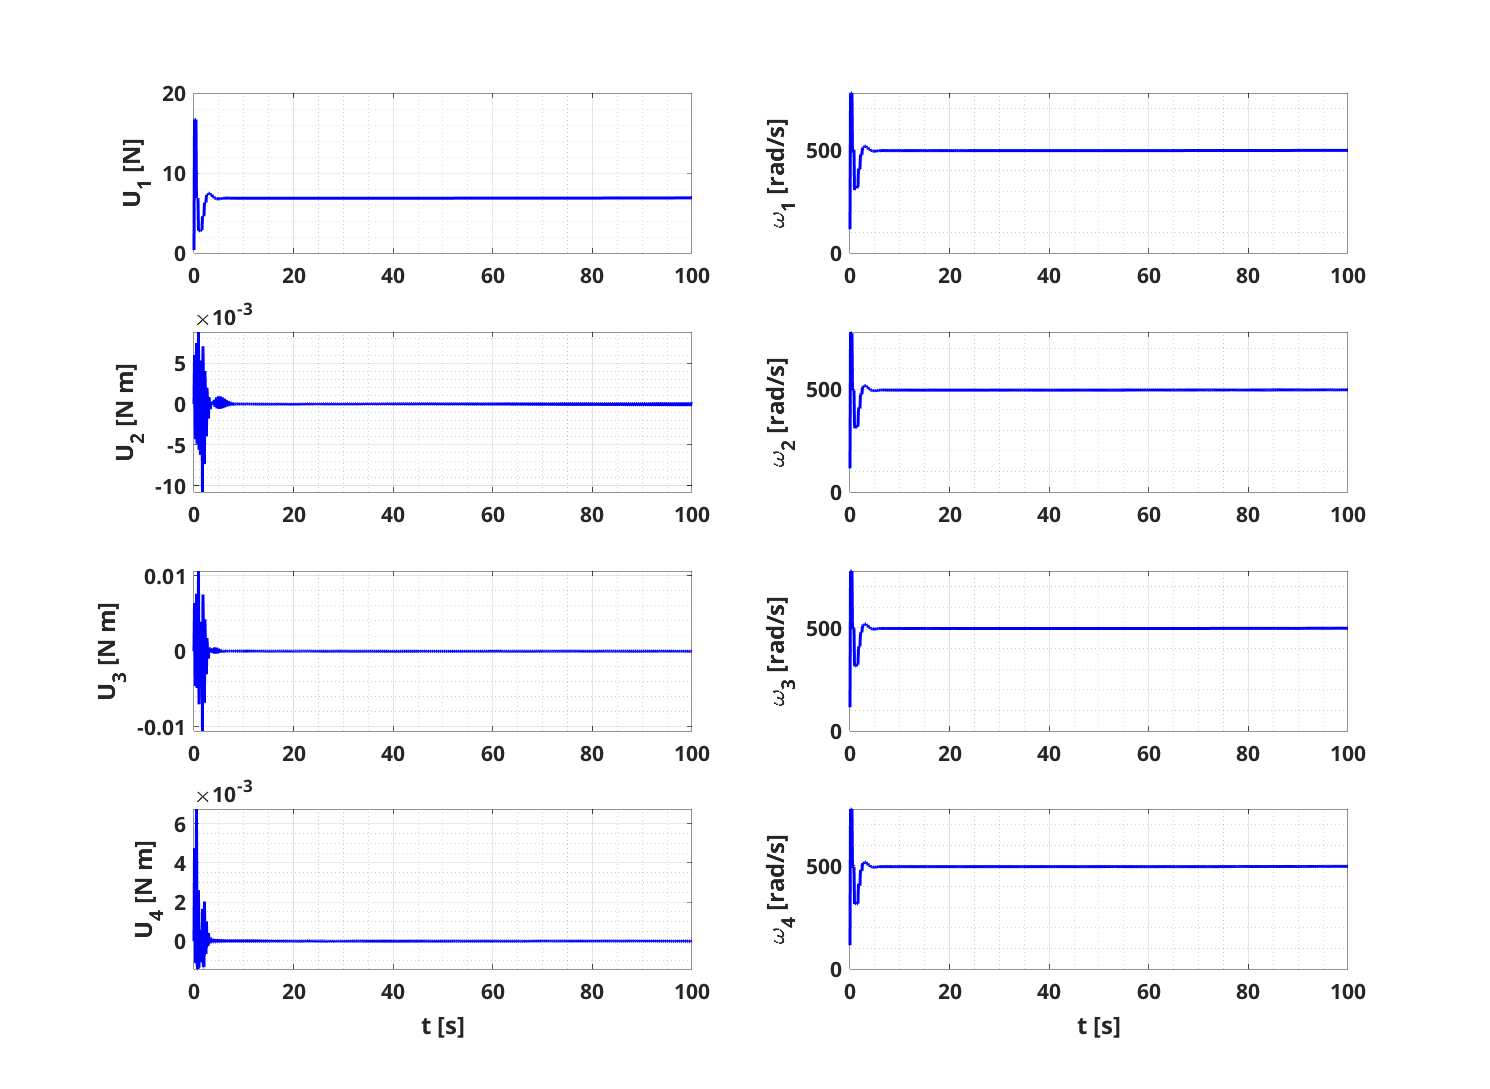
\includegraphics[width=0.95\textwidth]{traj6_inputs_rotors.png}
\caption{Trajectory 6: control inputs and rotor speeds.}
\end{figure}

\subsection{Trajectory 7: Straight diagonal run at constant speed with constant climb}\label{sec:t7}

This is the easiest case. The reference acceleration is zero, so after the start-up transient the roll and pitch angles are essentially zero, the yaw stays at a constant heading and the error settles to a small constant offset of about one decimeter. The inputs are constant.

\begin{figure}[H]
\centering
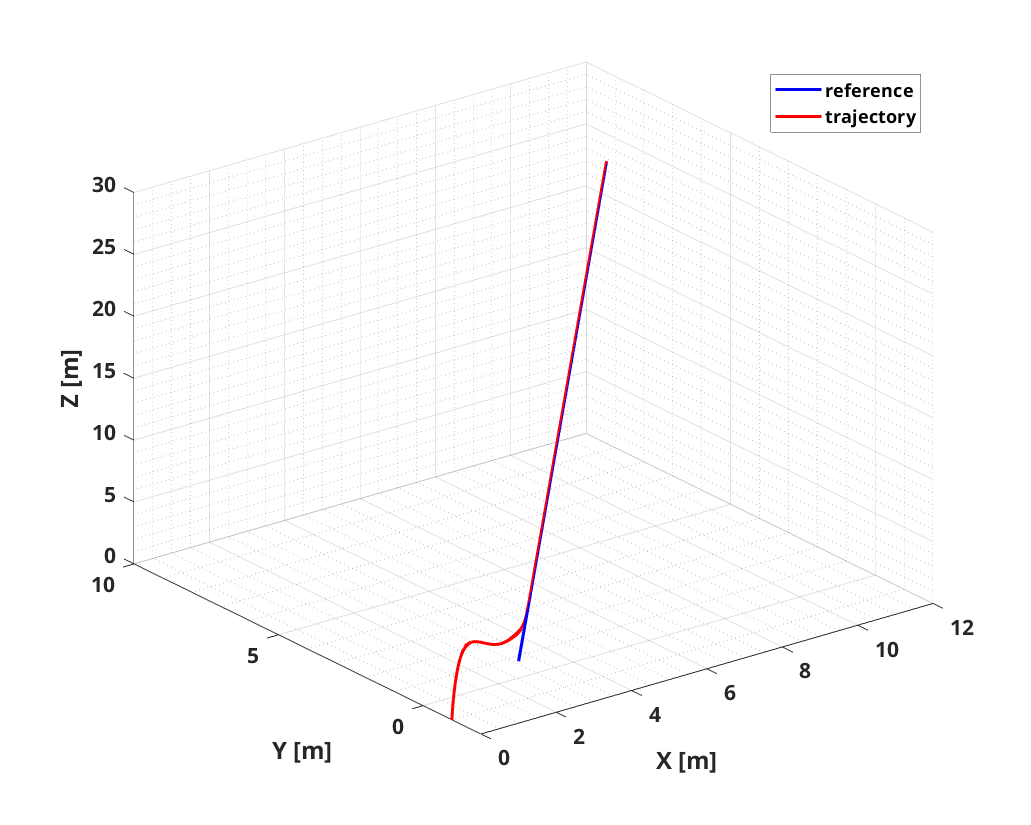
\includegraphics[width=0.72\textwidth]{traj7_path3d.png}
\caption{Trajectory 7: reference and flown path.}
\end{figure}

\begin{figure}[H]
\centering
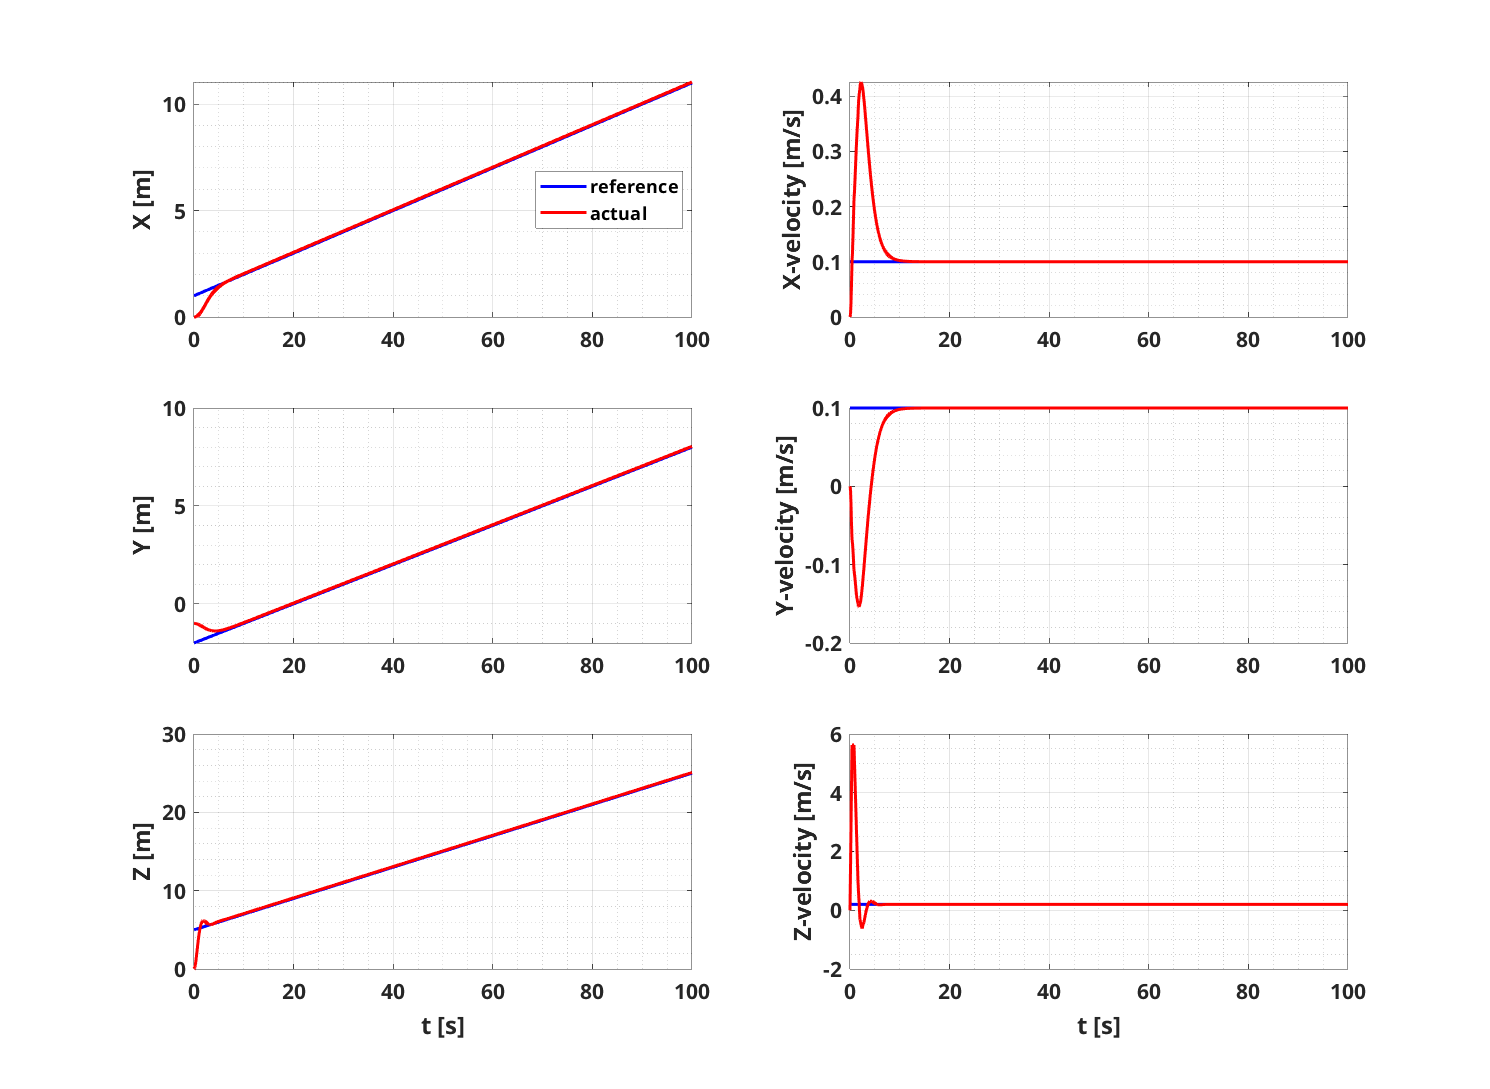
\includegraphics[width=0.95\textwidth]{traj7_position_velocity.png}
\caption{Trajectory 7: position and inertial velocity against reference.}
\end{figure}

\begin{figure}[H]
\centering
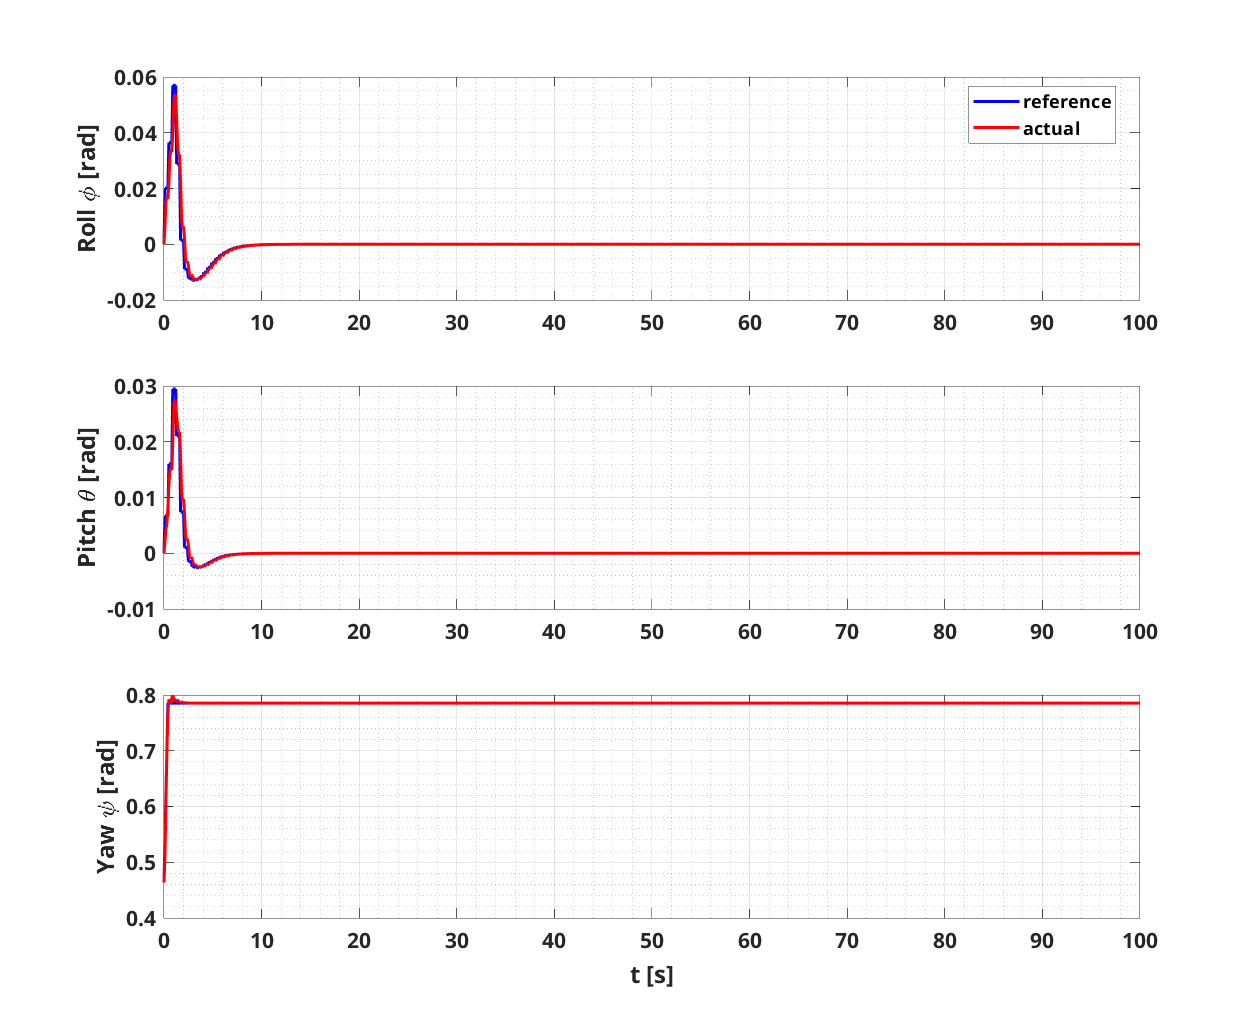
\includegraphics[width=0.95\textwidth]{traj7_attitude.png}
\caption{Trajectory 7: attitude angles against the references from the position loop.}
\end{figure}

\begin{figure}[H]
\centering
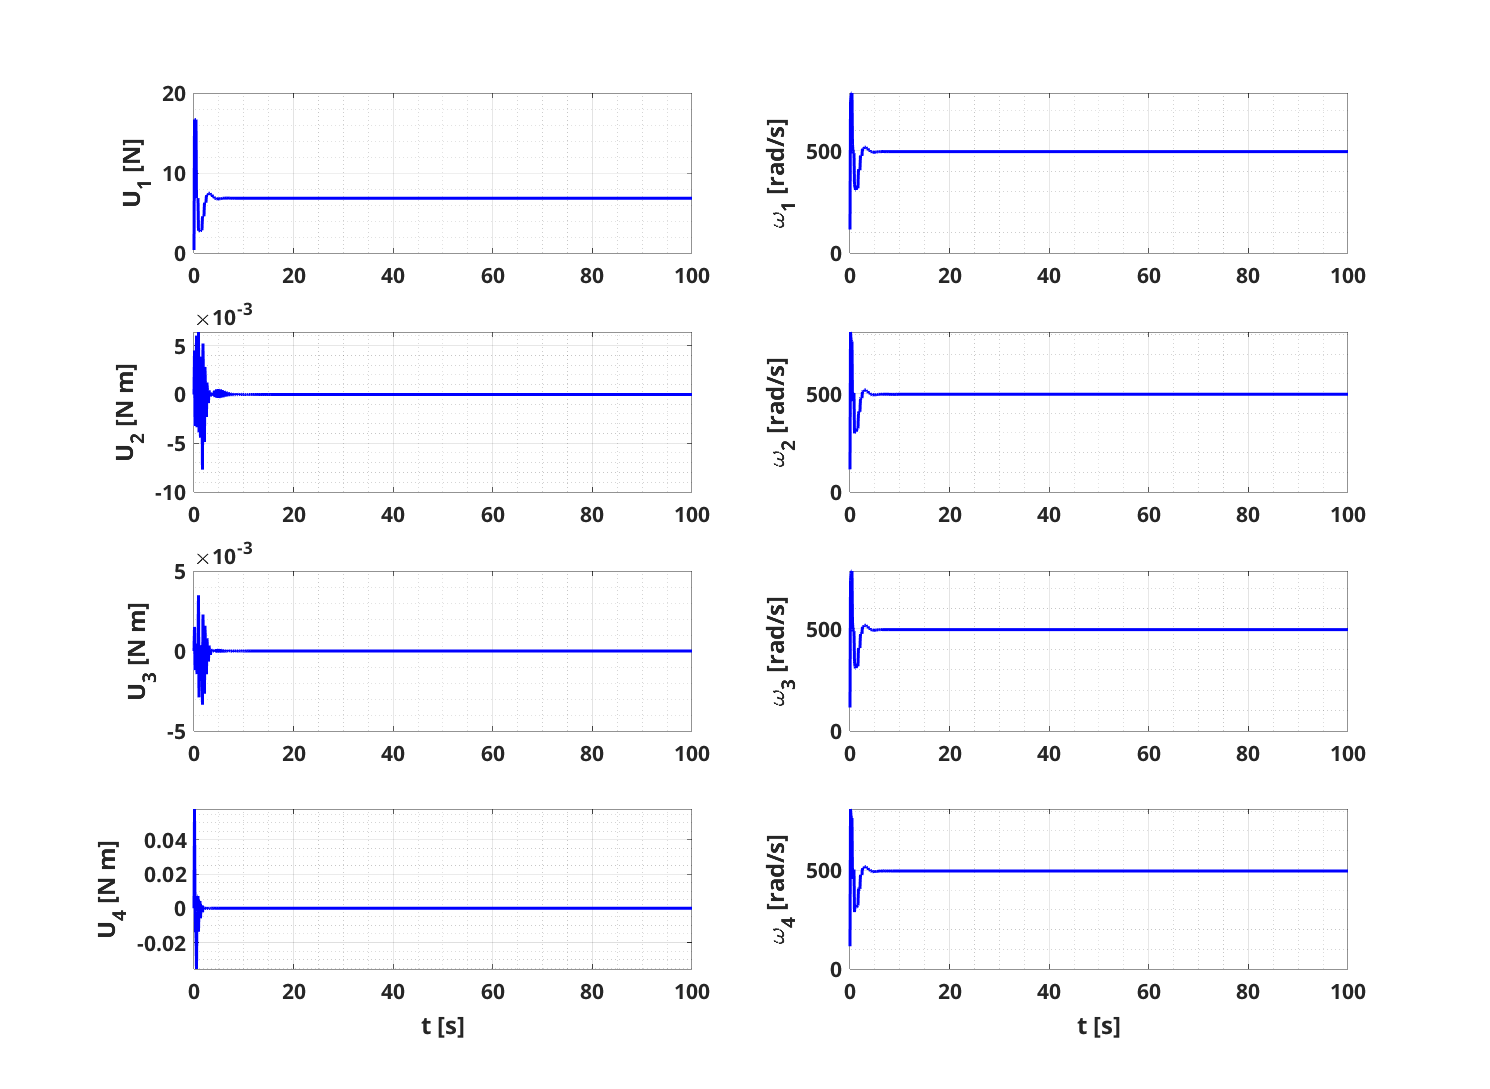
\includegraphics[width=0.95\textwidth]{traj7_inputs_rotors.png}
\caption{Trajectory 7: control inputs and rotor speeds.}
\end{figure}

\subsection{Trajectory 8: Weaving path with constant climb}\label{sec:t8}

The horizontal motion oscillates around a slowly drifting center, so the roll and pitch angles stay very small, but the heading of the path swings back and forth and the yaw reference follows it. The position error settles to a small constant offset of under a decimeter. The yaw torque shows bursts each time the heading reverses; the other inputs and the rotor speeds change very little.

\begin{figure}[H]
\centering
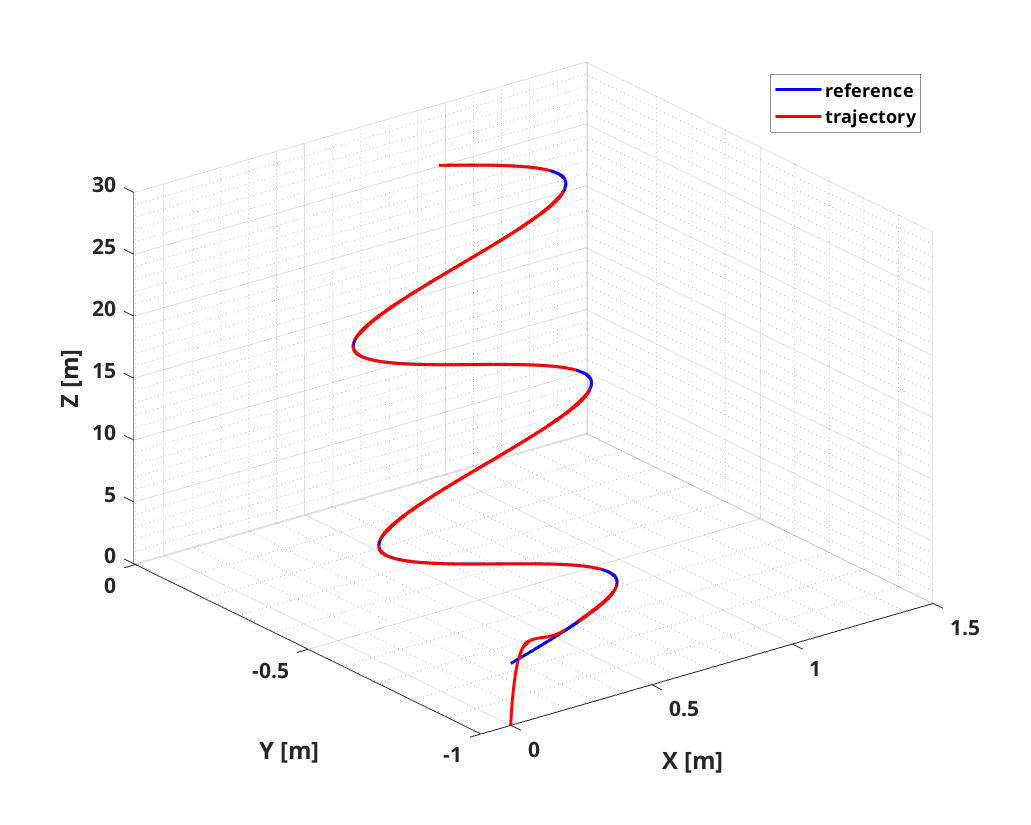
\includegraphics[width=0.72\textwidth]{traj8_path3d.png}
\caption{Trajectory 8: reference and flown path.}
\end{figure}

\begin{figure}[H]
\centering
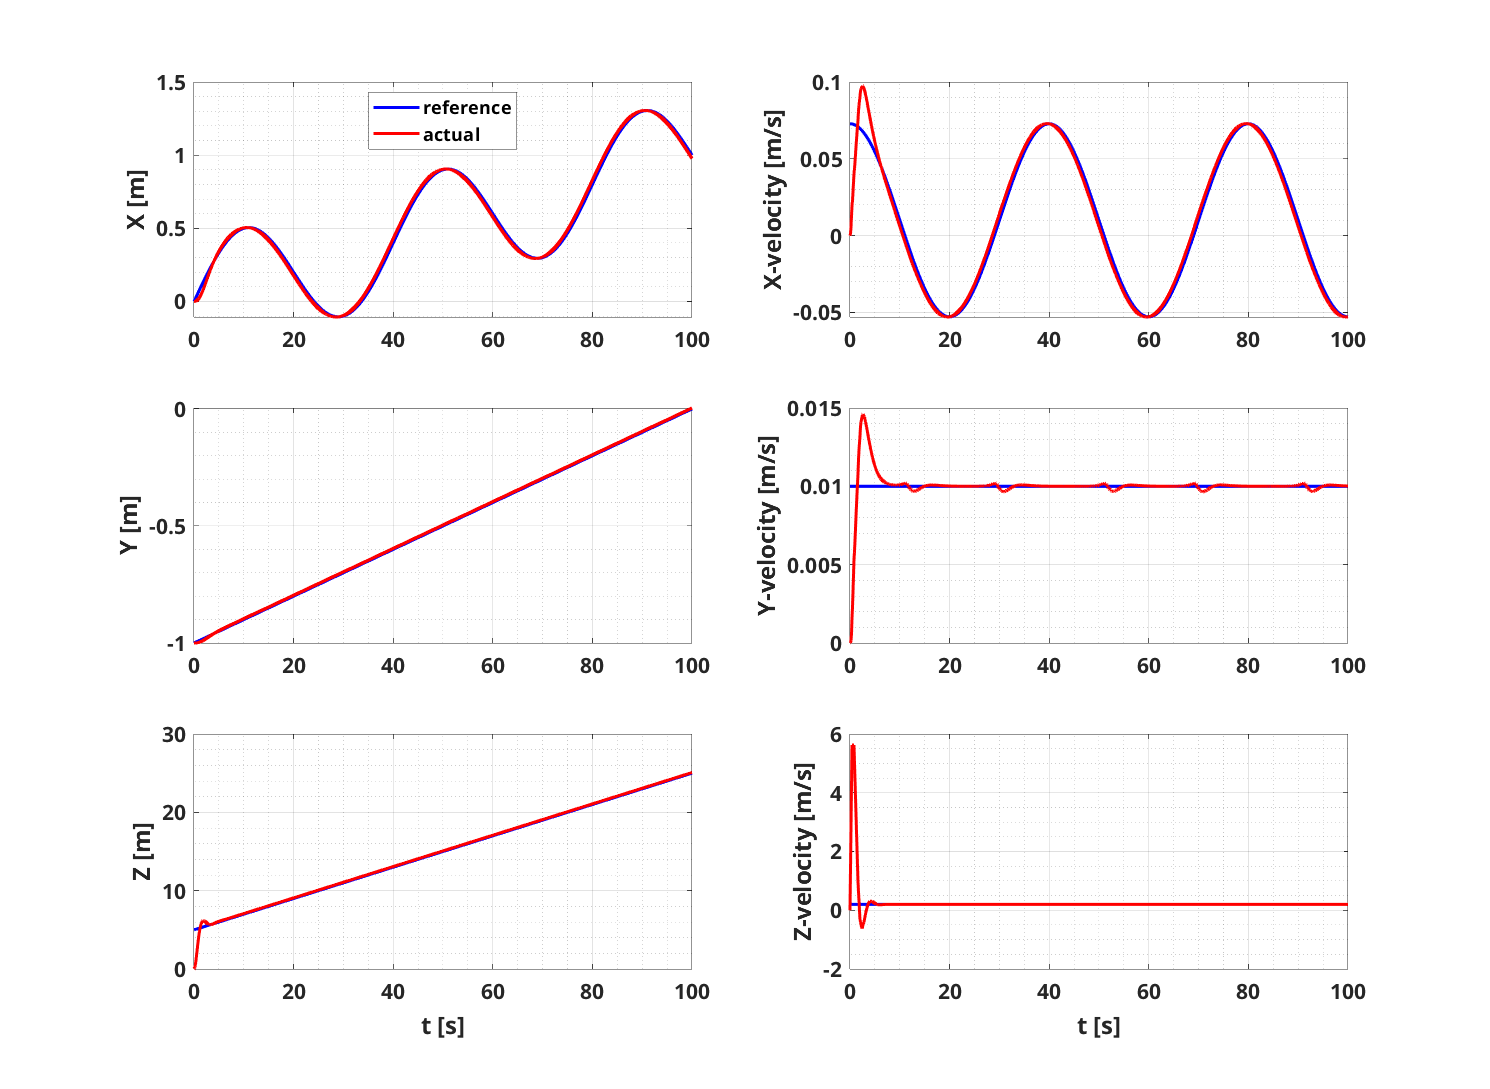
\includegraphics[width=0.95\textwidth]{traj8_position_velocity.png}
\caption{Trajectory 8: position and inertial velocity against reference.}
\end{figure}

\begin{figure}[H]
\centering
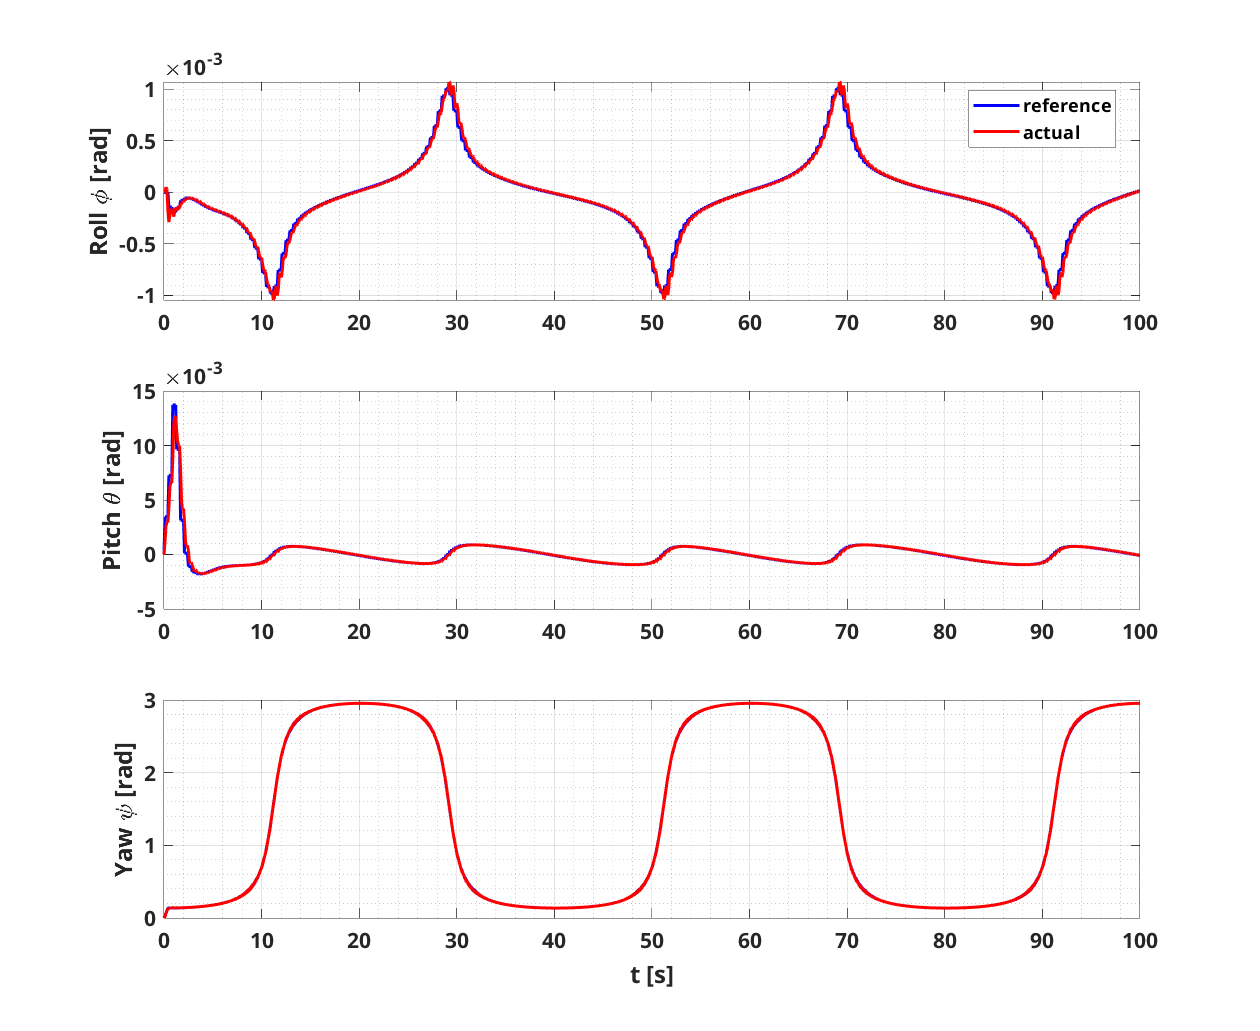
\includegraphics[width=0.95\textwidth]{traj8_attitude.png}
\caption{Trajectory 8: attitude angles against the references from the position loop.}
\end{figure}

\begin{figure}[H]
\centering
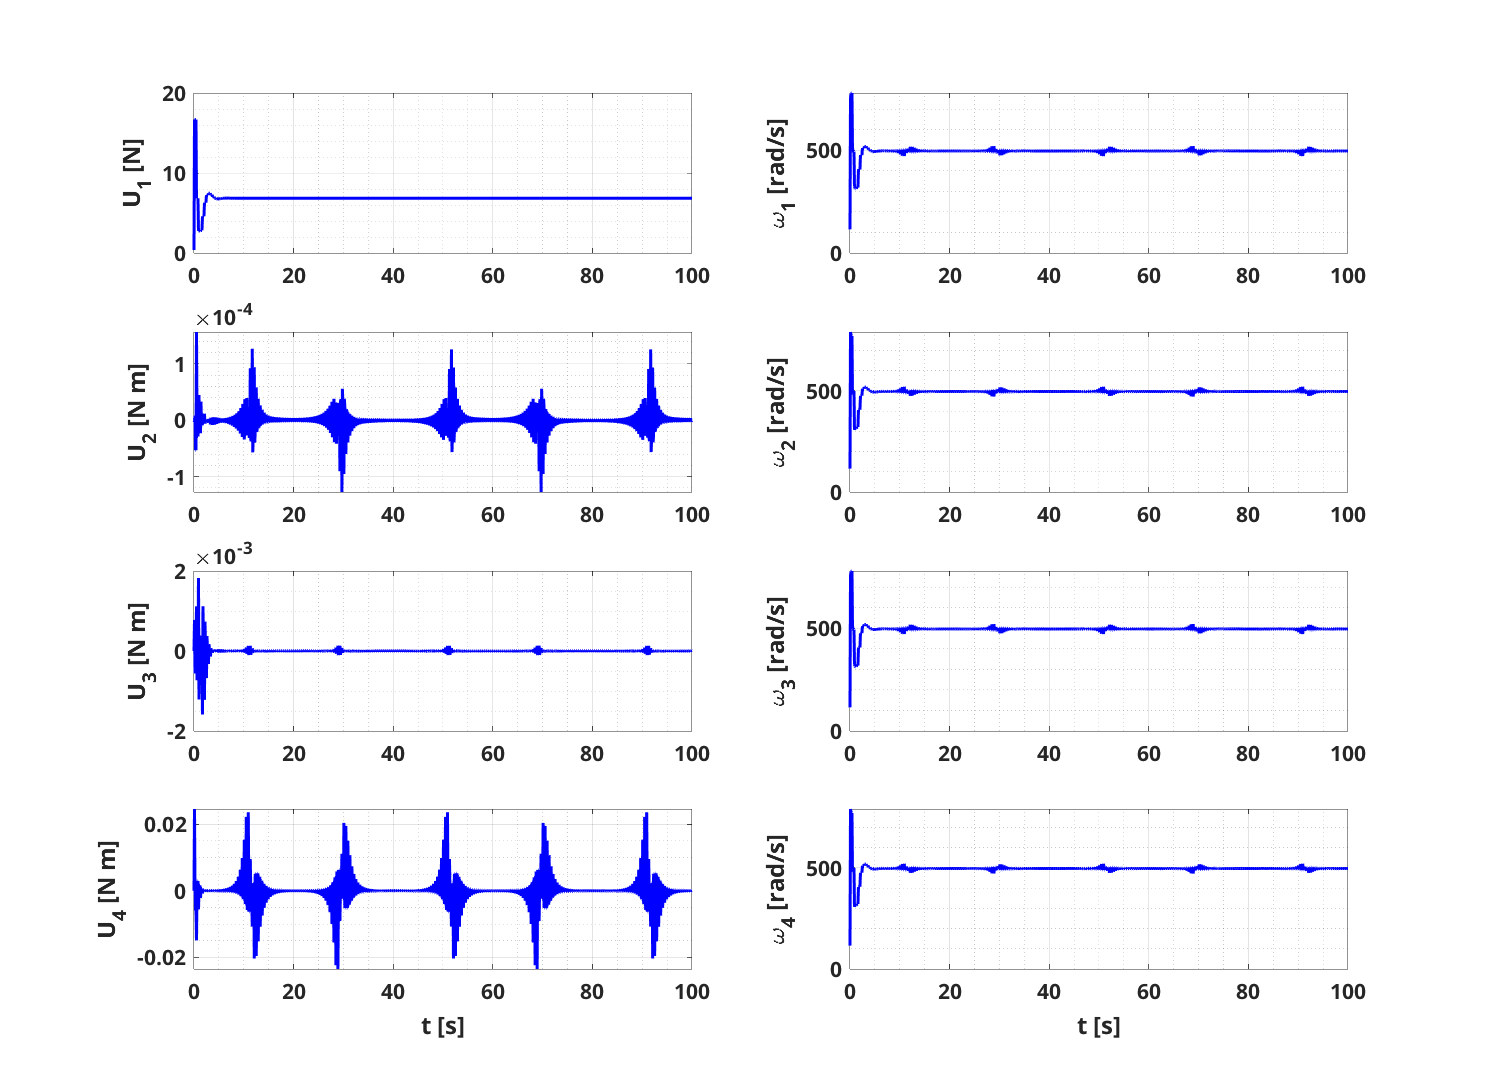
\includegraphics[width=0.95\textwidth]{traj8_inputs_rotors.png}
\caption{Trajectory 8: control inputs and rotor speeds.}
\end{figure}

\subsection{Trajectory 9: Circle with oscillating altitude}\label{sec:t9}

The vertical motion is oscillatory at a frequency well above that of the circular motion, so the thrust and the rotor speeds oscillate about their hover values for the whole run. The error oscillates at the same frequency with a peak of a few decimeters. This case also has the largest start-up tilt angles and the highest peak thrust, because the reference already has a large vertical speed and acceleration at the start.

\begin{figure}[H]
\centering
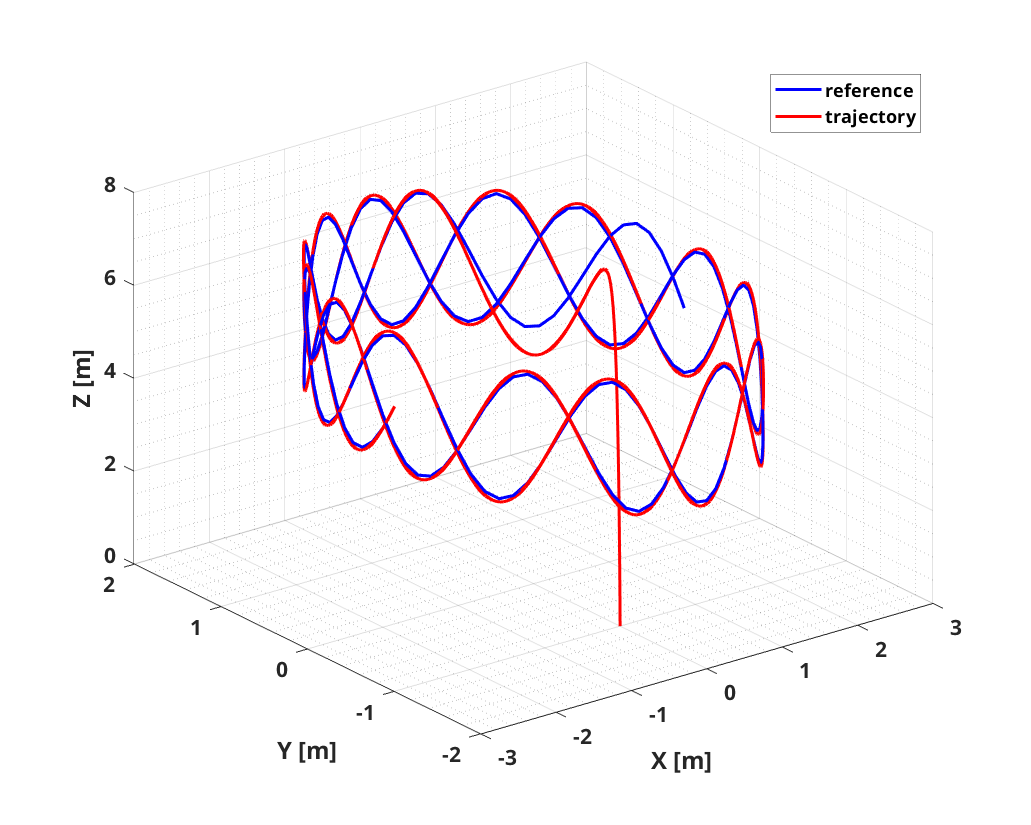
\includegraphics[width=0.72\textwidth]{traj9_path3d.png}
\caption{Trajectory 9: reference and flown path.}
\end{figure}

\begin{figure}[H]
\centering
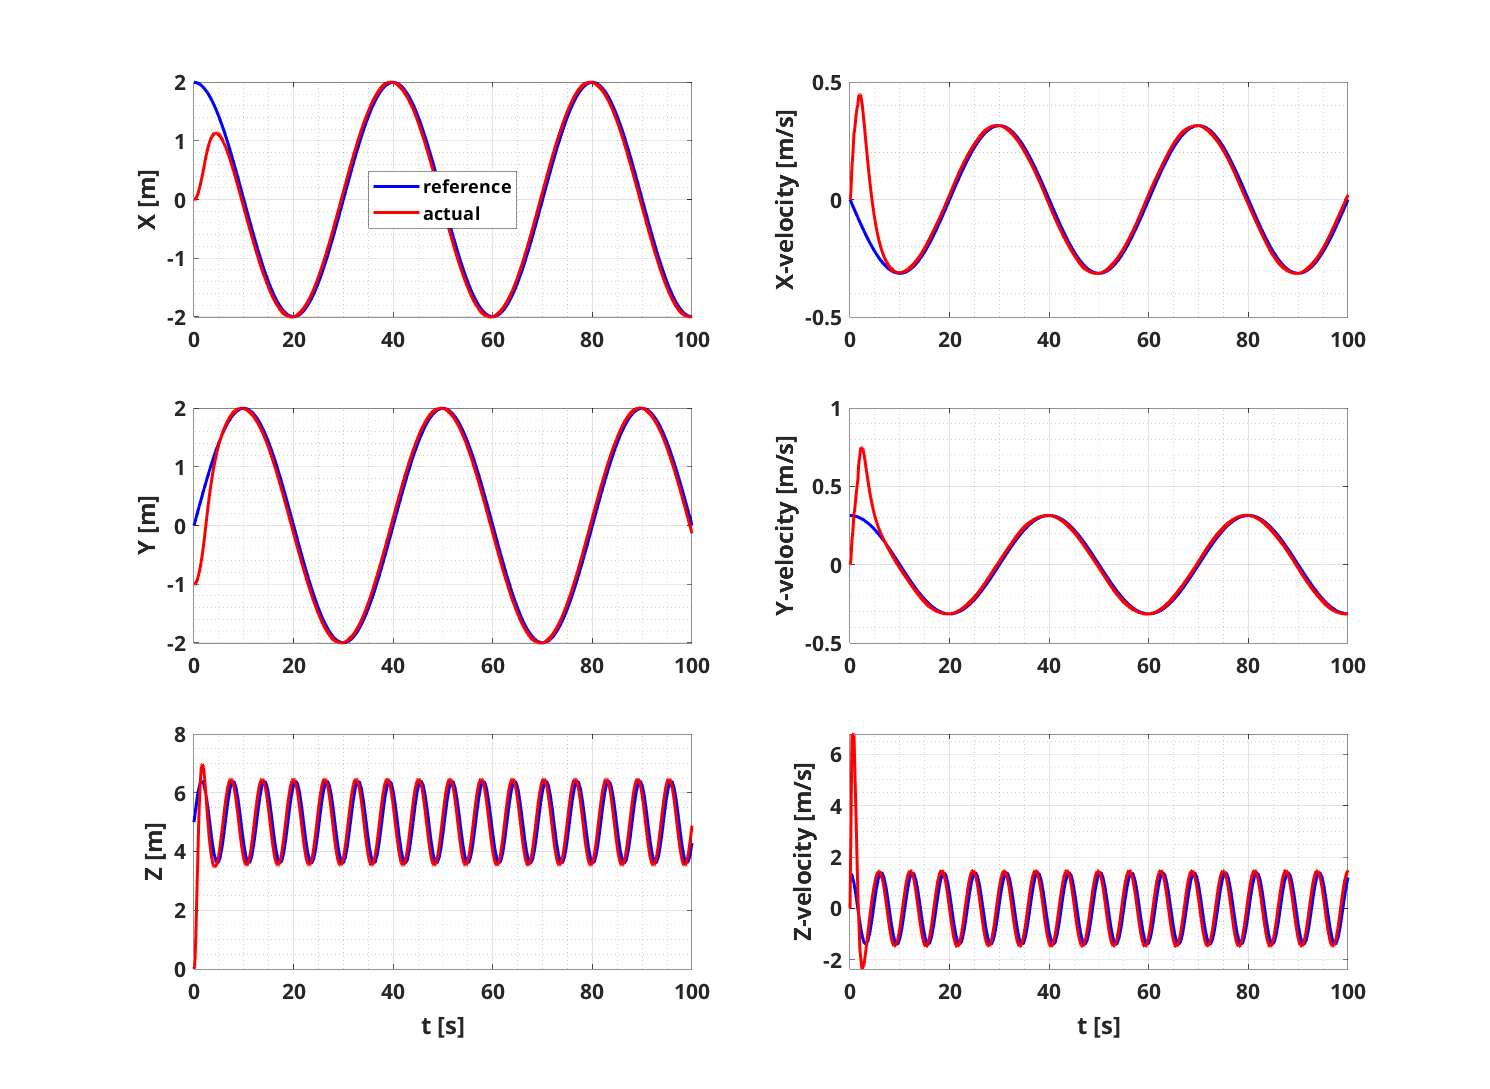
\includegraphics[width=0.95\textwidth]{traj9_position_velocity.png}
\caption{Trajectory 9: position and inertial velocity against reference.}
\end{figure}

\begin{figure}[H]
\centering
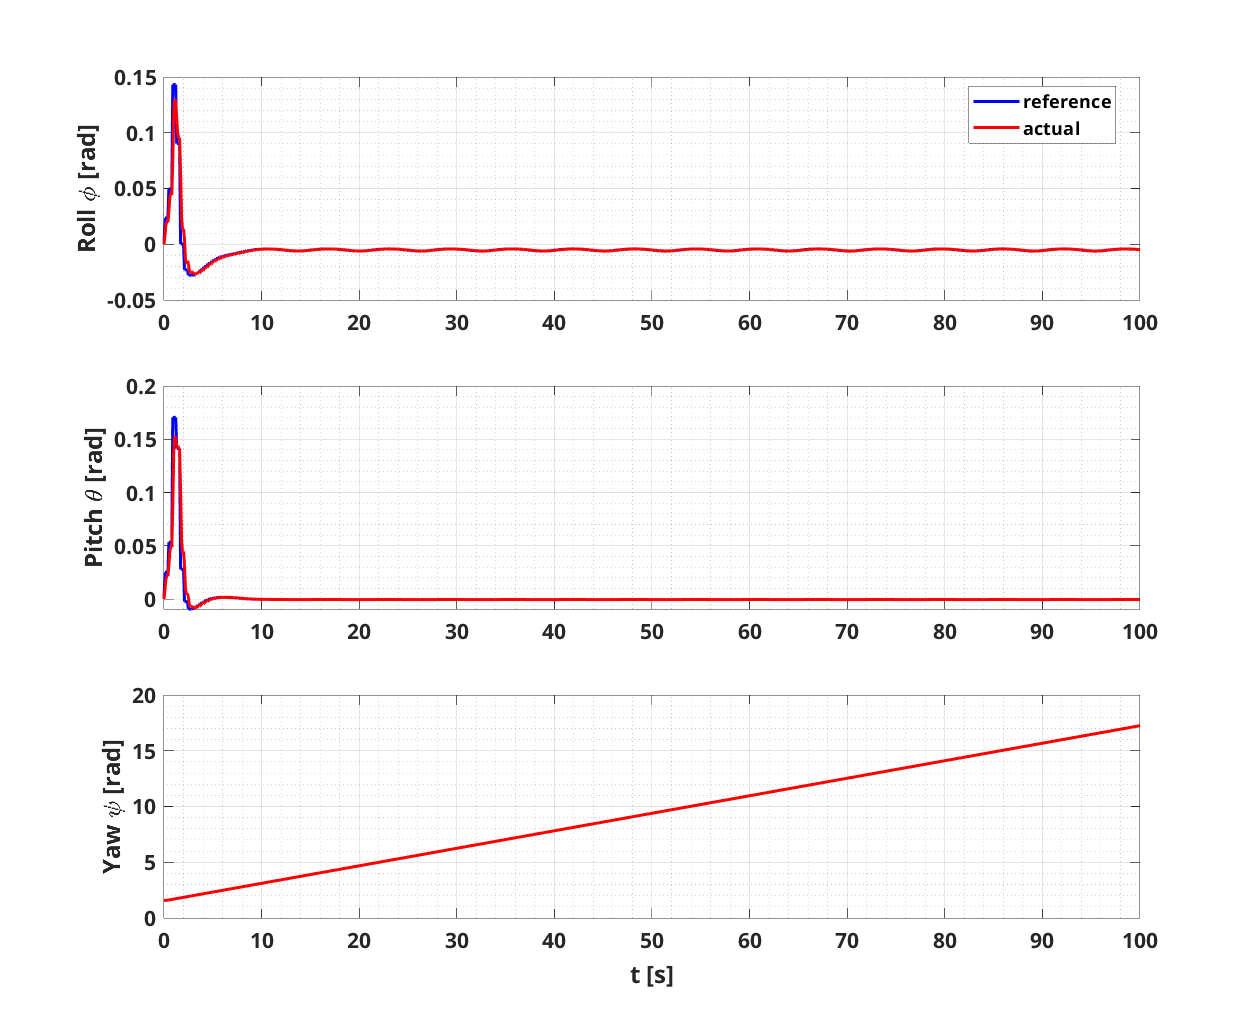
\includegraphics[width=0.95\textwidth]{traj9_attitude.png}
\caption{Trajectory 9: attitude angles against the references from the position loop.}
\end{figure}

\begin{figure}[H]
\centering
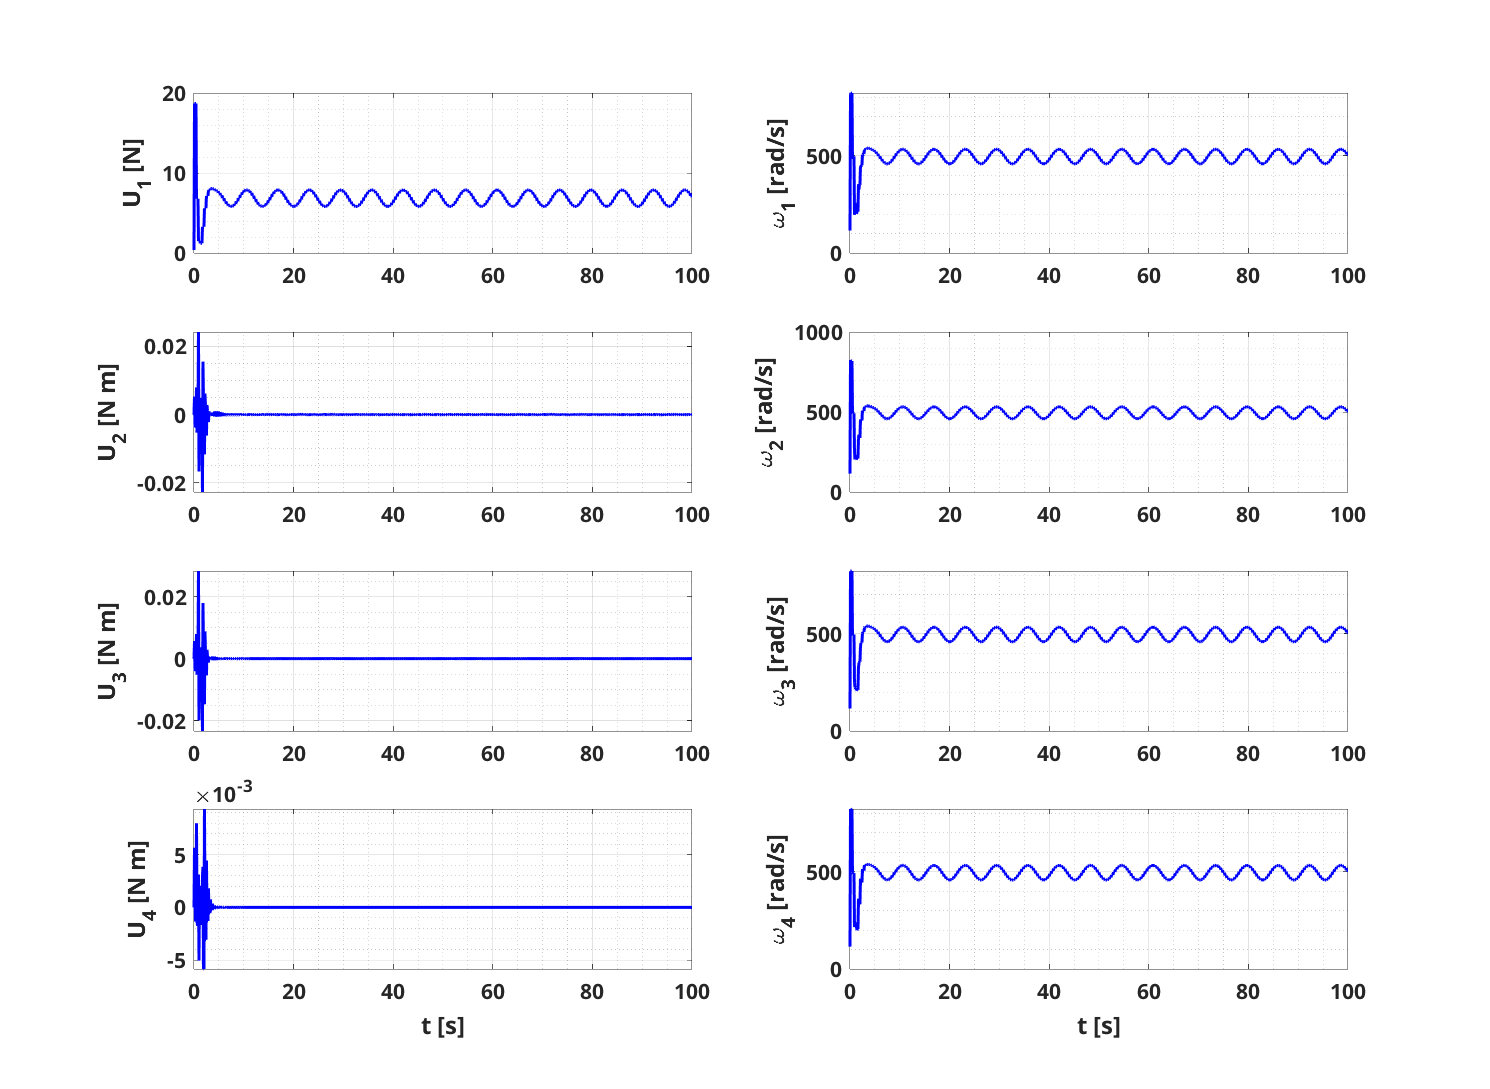
\includegraphics[width=0.95\textwidth]{traj9_inputs_rotors.png}
\caption{Trajectory 9: control inputs and rotor speeds.}
\end{figure}

\section{Limitations}\label{sec:limits}

The following limitations apply to the current implementation.

\begin{itemize}
\item The attitude controller has no constraints on torque, torque rate or rotor speed. The rotor speeds stay in a feasible range in all cases shown, but nothing in the controller enforces this.
\item The prediction model assumes small angles and freezes the scheduling parameters over the horizon. The model is therefore less accurate during aggressive maneuvers with large tilt.
\item Forward-Euler discretization of the prediction model is simple but only first-order accurate. This is acceptable at the sampling period used here and is the simplest choice that keeps the formulation transparent.
\item The position loop uses perfect state feedback. There is no sensor noise, estimation, wind disturbance or actuator dynamics.
\item The Euler-angle parameterization is singular at a pitch angle of $\pm 90^\circ$, so inverted or aggressive flips are outside the scope.
\item The mixer inversion requires positive squared rotor speeds, so a very large torque demand would make the inversion fail.
\end{itemize}

\section{Conclusion}\label{sec:conclusion}

A complete cascaded position and attitude controller for a quadrotor has been implemented and evaluated on nine trajectories. The position loop converts acceleration commands into thrust and tilt angles in closed form, and the attitude loop applies an unconstrained LPV model predictive controller whose solution is a single linear solve per sample. In closed loop, the vehicle recovers from a large initial offset within a few position periods and then tracks smooth trajectories to within a few decimeters or better, with rotor speeds and tilt angles in a moderate range. Expanding spirals and sudden changes in the reference acceleration produce the largest errors, and a continuously accelerating climb produces a lag that grows with the climb speed. Natural extensions are constraints in the predictive controller, a higher-order discretization, and disturbance and sensor models.

\begin{thebibliography}{9}
\bibitem{mellinger2011} D.~Mellinger and V.~Kumar, ``Minimum snap trajectory generation and control for quadrotors,'' in \emph{Proc.\ IEEE Int.\ Conf.\ Robotics and Automation}, 2011, pp.~2520--2525.
\bibitem{shamma1990} J.~S.~Shamma and M.~Athans, ``Analysis of gain scheduled control for nonlinear plants,'' \emph{IEEE Trans.\ Automatic Control}, vol.~35, no.~8, pp.~898--907, 1990.
\bibitem{briat2015} C.~Briat, \emph{Linear Parameter-Varying and Time-Delay Systems}. Berlin: Springer, 2015.
\bibitem{rawlings2017} J.~B.~Rawlings, D.~Q.~Mayne and M.~M.~Diehl, \emph{Model Predictive Control: Theory, Computation, and Design}, 2nd ed. Madison, WI: Nob Hill Publishing, 2017.
\bibitem{wang2009} L.~Wang, \emph{Model Predictive Control System Design and Implementation Using MATLAB}. London: Springer, 2009.
\bibitem{craig2005} J.~J.~Craig, \emph{Introduction to Robotics: Mechanics and Control}, 3rd ed. Upper Saddle River, NJ: Pearson Prentice Hall, 2005.
\bibitem{bouabdallah2004} S.~Bouabdallah, P.~Murrieri and R.~Siegwart, ``Design and control of an indoor micro quadrotor,'' in \emph{Proc.\ IEEE Int.\ Conf.\ Robotics and Automation}, 2004, pp.~4393--4398.
\bibitem{slotine1991} J.-J.~E.~Slotine and W.~Li, \emph{Applied Nonlinear Control}. Englewood Cliffs, NJ: Prentice Hall, 1991.
\end{thebibliography}

\end{document}
